% SMPdesign/SMPdesign.tex
% mainfile: ../perfbook.tex
% SPDX-License-Identifier: CC-BY-SA-3.0

\QuickQuizChapter{cha:Partitioning and Synchronization Design}{Partitioning and Synchronization Design}{qqzSMPdesign}
%
\Epigraph{Divide and rule.}{\emph{Philip II of Macedon}}

This chapter describes how to design software to take advantage of
modern commodity multicore systems by using idioms, or
``design patterns''~\cite{Alexander79,GOF95,SchmidtStalRohnertBuschmann2000v2Textbook},
to balance performance, scalability, and response time.
Correctly partitioned problems lead to simple, scalable, and
high-performance solutions, while poorly partitioned problems result
in slow and complex solutions.
This chapter will help you design partitioning into your code, with
some discussion of batching and weakening as well.
The word ``design'' is very important: You should partition first,
batch second, weaken third, and code fourth.
Changing this order often leads to poor performance and scalability
along with great frustration.\footnote{
	That other great dodge around the Laws of Physics, read-only
	replication, is covered in Chapter~\ref{chp:Deferred Processing}.}

To this end, Section~\ref{sec:SMPdesign:Partitioning Exercises}
presents partitioning exercises,
Section~\ref{sec:SMPdesign:Design Criteria} reviews partitionability
design criteria,
Section~\ref{sec:SMPdesign:Synchronization Granularity}
discusses synchronization granularity selection,
Section~\ref{sec:SMPdesign:Parallel Fastpath}
overviews important parallel-fastpath design patterns
that provide speed and scalability on common-case fastpaths while using
simpler less-scalable ``slow path'' fallbacks for unusual situations,
and finally
Section~\ref{sec:SMPdesign:Beyond Partitioning}
takes a brief look beyond partitioning.

% SMPdesign/partexercises.tex
% mainfile: ../perfbook.tex
% SPDX-License-Identifier: CC-BY-SA-3.0

\section{Partitioning Exercises}
\label{sec:SMPdesign:Partitioning Exercises}
%
\epigraph{Whenever a theory appears to you as the only possible one,
	  take this as a sign that you have neither understood the theory
	  nor the problem which it was intended to solve.}
	  {\emph{Karl Popper}}

Although partitioning is more widely understood than it was in the early
2000s, its value is still underappreciated.
\Cref{sec:SMPdesign:Dining Philosophers Problem}
therefore takes more highly parallel look at the classic Dining
Philosophers problem and
\cref{sec:SMPdesign:Double-Ended Queue}
revisits the double-ended queue.

\subsection{Dining Philosophers Problem}
\label{sec:SMPdesign:Dining Philosophers Problem}

\begin{figure}[tb]
\centering
\includegraphics[scale=.7]{SMPdesign/DiningPhilosopher5}
\caption{Dining Philosophers Problem}
\ContributedBy{Figure}{fig:SMPdesign:Dining Philosophers Problem}{Kornilios Kourtis}
\end{figure}

Figure~\ref{fig:SMPdesign:Dining Philosophers Problem} shows a diagram
of the classic \IX{Dining Philosophers problem}~\cite{Dijkstra1971HOoSP}.
This problem features five philosophers who do nothing but think and
eat a ``very difficult kind of spaghetti'' which requires two forks
to eat.\footnote{
	But feel free to instead think in terms of chopsticks.}
A given philosopher is permitted to use only the forks to his or her
immediate right and left, but will not put a given fork down until sated.

\begin{figure*}[tb]
\centering
\resizebox{5in}{!}{\includegraphics{cartoons/Dining-philosophers}}
\caption{Partial Starvation Is Also Bad}
\ContributedBy{Figure}{fig:cpu:Partial Starvation Is Also Bad}{Melissa Broussard}
\end{figure*}

The object is to construct an algorithm that, quite literally,
prevents starvation.
One starvation scenario would be if all of the philosophers picked up
their leftmost forks simultaneously.
Because none of them would put down their fork until after they ate,
and because none of them may pick up their second fork until at least
one has finished eating, they all starve.
Please note that it is not sufficient to allow at least one philosopher
to eat.
As Figure~\ref{fig:cpu:Partial Starvation Is Also Bad}
shows, starvation of even a few of the philosophers is to be avoided.

\begin{figure}[tb]
\centering
\includegraphics[scale=.7]{SMPdesign/DiningPhilosopher5TB}
\caption{Dining Philosophers Problem, Textbook Solution}
\ContributedBy{Figure}{fig:SMPdesign:Dining Philosophers Problem, Textbook Solution}{Kornilios Kourtis}
\end{figure}

\pplsur{Edsger W.}{Dijkstra}'s solution used a global semaphore,
which works fine assuming
negligible communications delays, an assumption that became invalid
in the late 1980s or early 1990s.\footnote{
	It is all too easy to denigrate Dijkstra from the viewpoint
	of the year 2012, more than 40 years after the fact.
	If you still feel the need to denigrate Dijkstra, my advice
	is to publish something, wait 40 years, and then see
	how well \emph{your} ideas stood the test of time.}
More recent solutions number the forks as shown in
Figure~\ref{fig:SMPdesign:Dining Philosophers Problem, Textbook Solution}.
Each philosopher picks up the lowest-numbered fork next to his or her
plate, then picks up the other fork.
The philosopher sitting in the uppermost position in the diagram thus
picks up the leftmost fork first, then the rightmost fork, while the
rest of the philosophers instead pick up their rightmost fork first.
Because two of the philosophers will attempt to pick up fork~1 first,
and because only one of those two philosophers will succeed,
there will be five forks available to four philosophers.
At least one of these four will have two forks, and will thus be able
to eat.

This general technique of numbering resources and acquiring them in
numerical order is heavily used as a deadlock-prevention technique.
However, it is easy to imagine a sequence of events that will result
in only one philosopher eating at a time even though all are hungry:

\begin{enumerate}
    \item P2 picks up fork~1, preventing P1 from taking a fork.
    \item P3 picks up fork~2.
    \item P4 picks up fork~3.
    \item P5 picks up fork~4.
    \item P5 picks up fork~5 and eats.
    \item P5 puts down forks~4 and 5.
    \item P4 picks up fork~4 and eats.
\end{enumerate}

In short, this algorithm can result in only one philosopher eating at
a given time, even when all five philosophers are hungry,
despite the fact that there are more than enough forks for two
philosophers to eat concurrently.
It should be possible to do better than this!

\begin{figure}[tb]
\centering
\includegraphics[scale=.7]{SMPdesign/DiningPhilosopher4part-b}
\caption{Dining Philosophers Problem, Partitioned}
\ContributedBy{Figure}{fig:SMPdesign:Dining Philosophers Problem, Partitioned}{Kornilios Kourtis}
\end{figure}

One approach is shown in
Figure~\ref{fig:SMPdesign:Dining Philosophers Problem, Partitioned},
which includes four philosophers rather than five to better illustrate the
partition technique.
Here the upper and rightmost philosophers share a pair of forks,
while the lower and leftmost philosophers share another pair of forks.
If all philosophers are simultaneously hungry, at least two will
always be able to eat concurrently.
In addition, as shown in the figure, the forks can now be bundled
so that the pair are picked up and put down simultaneously, simplifying
the acquisition and release algorithms.

\QuickQuiz{
	Is there a better solution to the Dining
	Philosophers Problem?
}\QuickQuizAnswer{
	One such improved solution is shown in
	Figure~\ref{fig:SMPdesign:Dining Philosophers Problem, Fully Partitioned},
	where the philosophers are simply provided with an additional
	five forks.
	All five philosophers may now eat simultaneously, and there
	is never any need for philosophers to wait on one another.
	In addition, this approach offers greatly improved disease control.

\begin{figure}[tb]
\centering
\includegraphics[scale=.7]{SMPdesign/DiningPhilosopher5PEM}
\caption{Dining Philosophers Problem, Fully Partitioned}
\QContributedBy{Figure}{fig:SMPdesign:Dining Philosophers Problem, Fully Partitioned}{Kornilios Kourtis}
\end{figure}

	This solution might seem like cheating to some, but such
	``cheating'' is key to finding good solutions to many
	concurrency problems.
}\QuickQuizEnd

This is an example of ``horizontal parallelism''~\cite{Inman85}
or ``data parallelism'',
so named because there is no dependency among the pairs of philosophers.
In a horizontally parallel data-processing system, a given item of data
would be processed by only one of a replicated set of software
components.

\QuickQuiz{
	And in just what sense can this ``horizontal parallelism'' be
	said to be ``horizontal''?
}\QuickQuizAnswer{
	Inman was working with protocol stacks, which are normally
	depicted vertically, with the application on top and the
	hardware interconnect on the bottom.
	Data flows up and down this stack.
	``Horizontal parallelism'' processes packets from different network
	connections in parallel, while ``vertical parallelism''
	handles different protocol-processing steps for a given
	packet in parallel.

	``Vertical parallelism'' is also called ``pipelining''.
}\QuickQuizEnd

\subsection{Double-Ended Queue}
\label{sec:SMPdesign:Double-Ended Queue}

A double-ended queue is a data structure containing a list of elements
that may be inserted or removed from either end~\cite{Knuth73}.
It has been claimed that a lock-based implementation permitting
concurrent operations on both ends of the double-ended queue is
difficult~\cite{DanGrossman2007TMGCAnalogy}.
This section shows how a partitioning design strategy can result
in a reasonably simple implementation, looking at three
general approaches in the following sections.

\subsubsection{Left- and Right-Hand Locks}
\label{sec:SMPdesign:Left- and Right-Hand Locks}

\begin{figure}[tb]
\centering
\resizebox{3in}{!}{\includegraphics{SMPdesign/lockdeq}}
\caption{Double-Ended Queue With Left- and Right-Hand Locks}
\label{fig:SMPdesign:Double-Ended Queue With Left- and Right-Hand Locks}
\end{figure}

One seemingly straightforward approach would be to use a doubly
linked list with a left-hand lock
for left-hand-end enqueue and dequeue operations along with a right-hand
lock for right-hand-end operations, as shown in
Figure~\ref{fig:SMPdesign:Double-Ended Queue With Left- and Right-Hand Locks}.
However, the problem with this approach is that the two locks'
domains must overlap when there are fewer than four elements on the
list.
This overlap is due to the fact that removing any given element affects
not only that element, but also its left- and right-hand neighbors.
These domains are indicated by color in the figure, with blue
with downward stripes indicating
the domain of the left-hand lock, red with upward stripes
indicating the domain of the right-hand
lock, and purple (with no stripes) indicating overlapping domains.
Although it is possible to create an algorithm that works this way,
the fact that it has no fewer than five special cases should raise
a big red flag, especially given that concurrent activity at the other
end of the list can shift the queue from one special case to another
at any time.
It is far better to consider other designs.

\subsubsection{Compound Double-Ended Queue}
\label{sec:SMPdesign:Compound Double-Ended Queue}

\begin{figure}[tb]
\centering
\resizebox{3in}{!}{\includegraphics{SMPdesign/lockdeqpair}}
\caption{Compound Double-Ended Queue}
\label{fig:SMPdesign:Compound Double-Ended Queue}
\end{figure}

One way of forcing non-overlapping lock domains is shown in
Figure~\ref{fig:SMPdesign:Compound Double-Ended Queue}.
Two separate double-ended queues are run in tandem, each protected by
its own lock.
This means that elements must occasionally be shuttled from one of
the double-ended queues to the other, in which case both locks must
be held.
A simple lock hierarchy may be used to avoid deadlock, for example,
always acquiring the left-hand lock before acquiring the right-hand lock.
This will be much simpler than applying two locks to the same
double-ended queue, as we can unconditionally left-enqueue elements
to the left-hand queue and right-enqueue elements to the right-hand
queue.
The main complication arises when dequeuing from an empty queue, in
which case it is necessary to:

\begin{enumerate}
\item	If holding the right-hand lock, release it and acquire the
	left-hand lock.
\item	Acquire the right-hand lock.
\item	Rebalance the elements across the two queues.
\item	Remove the required element if there is one.
\item	Release both locks.
\end{enumerate}

\QuickQuiz{
	In this compound double-ended queue implementation, what should
	be done if the queue has become non-empty while releasing
	and reacquiring the lock?
}\QuickQuizAnswer{
	In this case, simply dequeue an item from the non-empty
	queue, release both locks, and return.
}\QuickQuizEnd

The resulting code (\path{locktdeq.c}) is quite straightforward.
The rebalancing operation might well shuttle a given element back
and forth between the two queues, wasting time and possibly requiring
workload-dependent heuristics to obtain optimal performance.
Although this might well be the best approach in some cases, it is
interesting to try for an algorithm with greater determinism.

\subsubsection{Hashed Double-Ended Queue}
\label{sec:SMPdesign:Hashed Double-Ended Queue}

One of the simplest and most effective ways to deterministically
partition a data structure is to hash it.
It is possible to trivially hash a double-ended queue by assigning
each element a sequence number based on its position in the list,
so that the first element left-enqueued into an empty queue is numbered
zero and the first element right-enqueued into an empty queue is numbered
one.
A series of elements left-enqueued into an otherwise-idle queue would
be assigned decreasing numbers ($-1$, $-2$, $-3$, \ldots), while a series of
elements right-enqueued into an otherwise-idle queue would be assigned
increasing numbers (2, 3, 4, \ldots).
A key point is that it is not necessary to actually represent a given
element's number, as this number will be implied by its position in
the queue.

\begin{figure}[tb]
\centering
\resizebox{3in}{!}{\includegraphics{SMPdesign/lockdeqhash}}
\caption{Hashed Double-Ended Queue}
\label{fig:SMPdesign:Hashed Double-Ended Queue}
\end{figure}

Given this approach, we assign one lock to guard the left-hand index,
one to guard the right-hand index, and one lock for each hash chain.
Figure~\ref{fig:SMPdesign:Hashed Double-Ended Queue} shows the resulting
data structure given four hash chains.
Note that the lock domains do not overlap, and that deadlock is avoided
by acquiring the index locks before the chain locks, and by never
acquiring more than one lock of each type (index or chain) at a time.

\begin{figure}[tb]
\centering
\resizebox{3in}{!}{\includegraphics{SMPdesign/lockdeqhash1R}}
\caption{Hashed Double-Ended Queue After Insertions}
\label{fig:SMPdesign:Hashed Double-Ended Queue After Insertions}
\end{figure}

Each hash chain is itself a double-ended queue, and in this example,
each holds every fourth element.
The uppermost portion of
Figure~\ref{fig:SMPdesign:Hashed Double-Ended Queue After Insertions}
shows the state after a single element (``R$_1$'') has been
right-enqueued, with the right-hand index having been incremented to
reference hash chain~2.
The middle portion of this same figure shows the state after
three more elements have been right-enqueued.
As you can see, the indexes are back to their initial states
(see Figure~\ref{fig:SMPdesign:Hashed Double-Ended Queue}), however,
each hash chain is now non-empty.
The lower portion of this figure shows the state after three additional
elements have been left-enqueued and an additional element has been
right-enqueued.

From the last state shown in
Figure~\ref{fig:SMPdesign:Hashed Double-Ended Queue After Insertions},
a left-dequeue operation would return element ``L$_{-2}$'' and leave
the left-hand index referencing hash chain~2, which would then
contain only a single element (``R$_2$'').
In this state, a left-enqueue running concurrently with a right-enqueue
would result in lock contention, but the probability of such contention
can be reduced to arbitrarily low levels by using a larger hash table.

\begin{figure}[tb]
\centering
\resizebox{1.5in}{!}{\includegraphics{SMPdesign/lockdeqhashlots}}
\caption{Hashed Double-Ended Queue With 16 Elements}
\label{fig:SMPdesign:Hashed Double-Ended Queue With 16 Elements}
\end{figure}

Figure~\ref{fig:SMPdesign:Hashed Double-Ended Queue With 16 Elements}
shows how 16 elements would be organized in a four-hash-bucket
parallel double-ended queue.
Each underlying single-lock double-ended queue holds a one-quarter
slice of the full parallel double-ended queue.

\begin{listing}[tbp]
\input{CodeSamples/SMPdesign/lockhdeq@struct_pdeq.fcv}
\caption{Lock-Based Parallel Double-Ended Queue Data Structure}
\label{lst:SMPdesign:Lock-Based Parallel Double-Ended Queue Data Structure}
\end{listing}

Listing~\ref{lst:SMPdesign:Lock-Based Parallel Double-Ended Queue Data Structure}
shows the corresponding C-language data structure, assuming an
existing \co{struct deq} that provides a trivially locked
double-ended-queue implementation.
\begin{fcvref}[ln:SMPdesign:lockhdeq:struct_pdeq]
This data structure contains the left-hand lock on line~\lnref{llock},
the left-hand index on line~\lnref{lidx}, the right-hand lock on line~\lnref{rlock}
(which is cache-aligned in the actual implementation),
the right-hand index on line~\lnref{ridx}, and, finally, the hashed array
of simple lock-based double-ended queues on line~\lnref{bkt}.
A high-performance implementation would of course use padding or special
alignment directives to avoid false sharing.
\end{fcvref}

\begin{listing}[tbp]
\input{CodeSamples/SMPdesign/lockhdeq@pop_push.fcv}
\caption{Lock-Based Parallel Double-Ended Queue Implementation}
\label{lst:SMPdesign:Lock-Based Parallel Double-Ended Queue Implementation}
\end{listing}

Listing~\ref{lst:SMPdesign:Lock-Based Parallel Double-Ended Queue Implementation}
(\path{lockhdeq.c})
shows the implementation of the enqueue and dequeue functions.\footnote{
	One could easily create a polymorphic implementation in any
	number of languages, but doing so is left as an exercise for
	the reader.}
Discussion will focus on the left-hand operations, as the right-hand
operations are trivially derived from them.

\begin{fcvref}[ln:SMPdesign:lockhdeq:pop_push:popl]
\Clnrefrange{b}{e} show \co{pdeq_pop_l()},
which left\-/dequeues and returns
an element if possible, returning \co{NULL} otherwise.
Line~\lnref{acq} acquires the left-hand spinlock,
and line~\lnref{idx} computes the
index to be dequeued from.
Line~\lnref{deque} dequeues the element, and,
if line~\lnref{check} finds the result to be
non-\co{NULL}, line~\lnref{record} records the new left-hand index.
Either way, line~\lnref{rel} releases the lock, and,
finally, line~\lnref{return} returns
the element if there was one, or \co{NULL} otherwise.
\end{fcvref}

\begin{fcvref}[ln:SMPdesign:lockhdeq:pop_push:pushl]
\Clnrefrange{b}{e} show \co{pdeq_push_l()},
which left-enqueues the specified
element.
Line~\lnref{acq} acquires the left-hand lock,
and line~\lnref{idx} picks up the left-hand
index.
Line~\lnref{enque} left-enqueues the specified element
onto the double-ended queue
indexed by the left-hand index.
Line~\lnref{update} then updates the left-hand index
and line~\lnref{rel} releases the lock.
\end{fcvref}

As noted earlier, the right-hand operations are completely analogous
to their left-handed counterparts, so their analysis is left as an
exercise for the reader.

\QuickQuiz{
	Is the hashed double-ended queue a good solution?
	Why or why not?
}\QuickQuizAnswer{
	The best way to answer this is to run \path{lockhdeq.c} on
	a number of different multiprocessor systems, and you are
	encouraged to do so in the strongest possible terms.
	One reason for concern is that each operation on this
	implementation must acquire not one but two locks.
	% Getting about 500 nanoseconds per element when used as
	% a queue on a 4.2GHz Power system.  This is roughly the same as
	% the version covered by a single lock.  Sequential (unlocked
	% variant is more than an order of magnitude faster!

	The first well-designed performance study will be cited.\footnote{
		The studies by Dalessandro
		et al.~\cite{LukeDalessandro:2011:ASPLOS:HybridNOrecSTM:deque}
		and Dice et al.~\cite{DavidDice:2010:SCA:HTM:deque} are
		good starting points.}
	Do not forget to compare to a sequential implementation!
}\QuickQuizEnd

\subsubsection{Compound Double-Ended Queue Revisited}
\label{sec:SMPdesign:Compound Double-Ended Queue Revisited}

This section revisits the compound double-ended queue, using a trivial
rebalancing scheme that moves all the elements from the non-empty
queue to the now-empty queue.

\QuickQuiz{
	Move \emph{all} the elements to the queue that became empty?
	In what possible universe is this brain-dead solution in any
	way optimal???
}\QuickQuizAnswer{
	It is optimal in the case where data flow switches direction only
	rarely.
	It would of course be an extremely poor choice if the double-ended
	queue was being emptied from both ends concurrently.
	This of course raises another question, namely, in what possible
	universe emptying from both ends concurrently would be a reasonable
	thing to do.
	Work-stealing queues are one possible answer to this question.
}\QuickQuizEnd

In contrast to the hashed implementation presented in
the previous section, the compound implementation will build on
a sequential implementation of a double-ended queue that uses
neither locks nor atomic operations.

\begin{listing}[tbp]
\input{CodeSamples/SMPdesign/locktdeq@pop_push.fcv}
\caption{Compound Parallel Double-Ended Queue Implementation}
\label{lst:SMPdesign:Compound Parallel Double-Ended Queue Implementation}
\end{listing}

Listing~\ref{lst:SMPdesign:Compound Parallel Double-Ended Queue Implementation}
shows the implementation.
Unlike the hashed implementation, this compound implementation is
asymmetric, so that we must consider the \co{pdeq_pop_l()}
and \co{pdeq_pop_r()} implementations separately.

\QuickQuiz{
	Why can't the compound parallel double-ended queue
	implementation be symmetric?
}\QuickQuizAnswer{
	The need to avoid deadlock by imposing a lock hierarchy
	forces the asymmetry, just as it does in the fork-numbering
	solution to the Dining Philosophers Problem
	(see Section~\ref{sec:SMPdesign:Dining Philosophers Problem}).
}\QuickQuizEnd

\begin{fcvref}[ln:SMPdesign:locktdeq:pop_push:popl]
The \co{pdeq_pop_l()} implementation is shown on
\clnrefrange{b}{e}
of the figure.
Line~\lnref{acq:l} acquires the left-hand lock,
which line~\lnref{rel:l} releases.
Line~\lnref{deq:ll} attempts to left-dequeue an element
from the left-hand underlying
double-ended queue, and, if successful,
skips \clnrefrange{acq:r}{skip} to simply
return this element.
Otherwise, line~\lnref{acq:r} acquires the right-hand lock, line~\lnref{deq:lr}
left-dequeues an element from the right-hand queue,
and line~\lnref{move} moves any remaining elements on the right-hand
queue to the left-hand queue, line~\lnref{init:r} initializes
the right-hand queue,
and line~\lnref{rel:r} releases the right-hand lock.
The element, if any, that was dequeued on line~\lnref{deq:lr} will be returned.
\end{fcvref}

\begin{fcvref}[ln:SMPdesign:locktdeq:pop_push:popr]
The \co{pdeq_pop_r()} implementation is shown on \clnrefrange{b}{e}
of the figure.
As before, line~\lnref{acq:r1} acquires the right-hand lock
(and line~\lnref{rel:r2}
releases it), and line~\lnref{deq:rr1} attempts to right-dequeue an element
from the right-hand queue, and, if successful,
skips \clnrefrange{rel:r1}{skip2}
to simply return this element.
However, if line~\lnref{check1} determines that there was no element to dequeue,
line~\lnref{rel:r1} releases the right-hand lock and
\clnrefrange{acq:l}{acq:r2} acquire both
locks in the proper order.
Line~\lnref{deq:rr2} then attempts to right-dequeue an element
from the right-hand
list again, and if line~\lnref{check2} determines that this second attempt has
failed, line~\lnref{deq:rl} right-dequeues an element from the left-hand queue
(if there is one available), line~\lnref{move} moves any remaining elements
from the left-hand queue to the right-hand queue, and line~\lnref{init:l}
initializes the left-hand queue.
Either way, line~\lnref{rel:l} releases the left-hand lock.
\end{fcvref}

\QuickQuizSeries{%
\QuickQuizB{
	Why is it necessary to retry the right-dequeue operation
	on line~\ref{ln:SMPdesign:locktdeq:pop_push:popr:deq:rr2} of
	Listing~\ref{lst:SMPdesign:Compound Parallel Double-Ended Queue Implementation}?
}\QuickQuizAnswerB{
	\begin{fcvref}[ln:SMPdesign:locktdeq:pop_push:popr]
	This retry is necessary because some other thread might have
	enqueued an element between the time that this thread dropped
	\co{d->rlock} on line~\lnref{rel:r1} and the time that it reacquired this
	same lock on line~\lnref{acq:r2}.
	\end{fcvref}
}\QuickQuizEndB
%
\QuickQuizE{
	Surely the left-hand lock must \emph{sometimes} be available!!!
	So why is it necessary that
        line~\ref{ln:SMPdesign:locktdeq:pop_push:popr:rel:r1} of
	Listing~\ref{lst:SMPdesign:Compound Parallel Double-Ended Queue Implementation}
	unconditionally release the right-hand lock?
}\QuickQuizAnswerE{
	It would be possible to use \co{spin_trylock()} to attempt
	to acquire the left-hand lock when it was available.
	However, the failure case would still need to drop the
	right-hand lock and then re-acquire the two locks in order.
	Making this transformation (and determining whether or not
	it is worthwhile) is left as an exercise for the reader.
}\QuickQuizEndE
}

\begin{fcvref}[ln:SMPdesign:locktdeq:pop_push:pushl]
The \co{pdeq_push_l()} implementation is shown on
\clnrefrange{b}{e} of
Listing~\ref{lst:SMPdesign:Compound Parallel Double-Ended Queue Implementation}.
Line~\lnref{acq:l} acquires the left-hand spinlock,
line~\lnref{que:l} left-enqueues the
element onto the left-hand queue, and finally line~\lnref{rel:l} releases
the lock.
\end{fcvref}
\begin{fcvref}[ln:SMPdesign:locktdeq:pop_push:pushr]
The \co{pdeq_push_r()} implementation (shown on \clnrefrange{b}{e})
is quite similar.
\end{fcvref}

\QuickQuiz{
	But in the case where data is flowing in only one direction,
	the algorithm shown in
	Listing~\ref{lst:SMPdesign:Compound Parallel Double-Ended Queue Implementation}
	will have both ends attempting to acquire the same lock
	whenever the consuming end empties its underlying
	double-ended queue.
	Doesn't that mean that sometimes this algorithm fails to
	provide concurrent access to both ends of the queue even
	when the queue contains an arbitrarily large number of elements?
}\QuickQuizAnswer{
	Indeed it does!

	But the same is true of other algorithms claiming this property.
	For example, in solutions using software transactional memory
	mechanisms based on hashed arrays of locks,
	the leftmost and rightmost elements' addresses will sometimes
	happen to hash to the same lock.
	These hash collisions will also prevent concurrent access.
	For another example, solutions using hardware transactional
	memory mechanisms with software
	fallbacks~\cite{Yoo:2013:PEI:2503210.2503232,RickMerrit2011PowerTM,ChristianJacobi2012MainframeTM}
	often use locking within those software fallbacks, and thus
	suffer (albeit hopefully rarely) from whatever concurrency
	limitations that these locking solutions suffer from.

	Therefore, as of last 2017, all practical solutions to the
	concurrent double-ended queue problem fail to provide full
	concurrency in at least some circumstances, including the
	compound double-ended queue.
}\QuickQuizEnd

\subsubsection{Double-Ended Queue Discussion}
\label{sec:SMPdesign:Double-Ended Queue Discussion}

The compound implementation is somewhat more complex than the
hashed variant presented in
Section~\ref{sec:SMPdesign:Hashed Double-Ended Queue},
but is still reasonably simple.
Of course, a more intelligent rebalancing scheme could be arbitrarily
complex, but the simple scheme shown here has been shown to
perform well compared to software
alternatives~\cite{LukeDalessandro:2011:ASPLOS:HybridNOrecSTM:deque}
and even compared to algorithms using hardware
assist~\cite{DavidDice:2010:SCA:HTM:deque}.
Nevertheless, the best we can hope for from such a scheme
is 2x scalability, as at most two threads can be holding the
dequeue's locks concurrently.
This limitation also applies to algorithms based on non-blocking
synchronization, such as the compare-and-swap-based dequeue algorithm of
Michael~\cite{DBLP:conf/europar/Michael03}.\footnote{
	This paper is interesting in that it showed that special
	double-compare-and-swap (DCAS) instructions are not needed
	for lock-free implementations of double-ended queues.
	Instead, the common compare-and-swap (e.g., x86 cmpxchg)
	suffices.}

\QuickQuiz{
	Why are there not one but two solutions to the double-ended queue
	problem?
}\QuickQuizAnswer{
	There are actually at least three.
	The third, by Dominik Dingel, makes interesting use of
	reader-writer locking, and may be found in \path{lockrwdeq.c}.
}\QuickQuizEnd

In fact, as noted by Dice et al.~\cite{DavidDice:2010:SCA:HTM:deque},
an unsynchronized single-threaded double-ended queue significantly
outperforms any of the parallel implementations they studied.
Therefore, the key point is that there can be significant overhead enqueuing to
or dequeuing from a shared queue, regardless of implementation.
This should come as no surprise given the material in
Chapter~\ref{chp:Hardware and its Habits}, given the strict
first-in-first-out (FIFO) nature of these queues.

Furthermore, these strict FIFO queues are strictly FIFO only with
respect to
\emph{linearization points}~\cite{Herlihy:1990:LCC:78969.78972}\footnote{
	In short, a linearization point is a single point within a given
	function where that function can be said to have taken effect.
	In this lock-based implementation, the linearization points
	can be said to be anywhere within the critical section that
	does the work.}
that are not visible to the caller, in fact, in these examples,
the linearization points are buried in the lock-based critical
sections.
These queues are not strictly FIFO with respect to (say) the times at which
the individual operations started~\cite{AndreasHaas2012FIFOisnt}.
This indicates that the strict FIFO property is not all that valuable
in concurrent programs, and in fact, Kirsch et al.~present less-strict
queues that provide improved performance and
scalability~\cite{ChristophMKirsch2012FIFOisntTR}.\footnote{
	Nir Shavit produced relaxed stacks for roughly the same
	reasons~\cite{Shavit:2011:DSM:1897852.1897873}.
	This situation leads some to believe that the linearization
	points are useful to theorists rather than developers, and
	leads others to wonder to what extent the designers of such
	data structures and algorithms were considering the needs
	of their users.}
All that said, if you are pushing all the data used by your concurrent
program through a single queue, you really need to rethink your
overall design.

\subsection{Partitioning Example Discussion}
\label{sec:SMPdesign:Partitioning Example Discussion}

The optimal solution to the dining philosophers problem given in
the answer to the Quick Quiz in
Section~\ref{sec:SMPdesign:Dining Philosophers Problem}
is an excellent example of ``horizontal parallelism'' or
``data parallelism''.
The synchronization overhead in this case is nearly (or even exactly)
zero.
In contrast, the double-ended
queue implementations are examples of ``vertical parallelism'' or
``pipelining'', given that data moves from one thread to another.
The tighter coordination required for pipelining in turn requires
larger units of work to obtain a given level of efficiency.

\QuickQuizSeries{%
\QuickQuizB{
	The tandem double-ended queue runs about twice as fast as
	the hashed double-ended queue, even when I increase the
	size of the hash table to an insanely large number.
	Why is that?
}\QuickQuizAnswerB{
	The hashed double-ended queue's locking design only permits
	one thread at a time at each end, and further requires
	two lock acquisitions for each operation.
	The tandem double-ended queue also permits one thread at a time
	at each end, and in the common case requires only one lock
	acquisition per operation.
	Therefore, the tandem double-ended queue should be expected to
	outperform the hashed double-ended queue.

	Can you create a double-ended queue that allows multiple
	concurrent operations at each end?
	If so, how?  If not, why not?
}\QuickQuizEndB
%
\QuickQuizE{
	Is there a significantly better way of handling concurrency
	for double-ended queues?
}\QuickQuizAnswerE{
	One approach is to transform the problem to be solved
	so that multiple double-ended queues can be used in parallel,
	allowing the simpler single-lock double-ended queue to be used,
	and perhaps also replace each double-ended queue with a pair of
	conventional single-ended queues.
	Without such ``horizontal scaling'', the speedup is limited
	to 2.0.
	In contrast, horizontal-scaling designs can achieve very large
	speedups, and are especially attractive if there are multiple threads
	working either end of the queue, because in this
	multiple-thread case the dequeue
	simply cannot provide strong ordering guarantees.
	After all, the fact that a given thread removed an item first
	in no way implies that it will process that item
	first~\cite{AndreasHaas2012FIFOisnt}.
	And if there are no guarantees, we may as well obtain the
	performance benefits that come with refusing to provide these
	guarantees.
	% about twice as fast as hashed version on 4.2GHz Power.

	Regardless of whether or not the problem can be transformed
	to use multiple queues, it is worth asking whether work can
	be batched so that each enqueue and dequeue operation corresponds
	to larger units of work.
	This batching approach decreases contention on the queue data
	structures, which increases both performance and scalability,
	as will be seen in
	Section~\ref{sec:SMPdesign:Synchronization Granularity}.
	After all, if you must incur high synchronization overheads,
	be sure you are getting your money's worth.

	Other researchers are working on other ways to take advantage
	of limited ordering guarantees in
	queues~\cite{ChristophMKirsch2012FIFOisntTR}.
}\QuickQuizEndE
}

These two examples show just how powerful partitioning can be in
devising parallel algorithms.
Section~\ref{sec:SMPdesign:Locking Granularity and Performance}
looks briefly at a third example, matrix multiply.
However, all three of these examples beg for more and better design
criteria for parallel programs, a topic taken up in the next section.


% SMPdesign/criteria.tex
% mainfile: ../perfbook.tex
% SPDX-License-Identifier: CC-BY-SA-3.0

\section{Design Criteria}
\label{sec:SMPdesign:Design Criteria}
%
\epigraph{One pound of learning requires ten pounds of commonsense to apply it.}
	 {\emph{Persian proverb}}

One way to obtain the best performance and scalability is to simply
hack away until you converge on the best possible parallel program.
Unfortunately, if your program is other than microscopically tiny,
the space of possible parallel programs is so huge
that convergence is not guaranteed in the lifetime of the universe.
Besides, what exactly is the ``best possible parallel program''?
After all, Section~\ref{sec:intro:Parallel Programming Goals}
called out no fewer than three parallel-programming goals of
performance, productivity, and generality,
and the best possible performance will likely come at a cost in
terms of productivity and generality.
We clearly need to be able to make higher-level choices at design
time in order to arrive at an acceptably good parallel program
before that program becomes obsolete.

However, more detailed design criteria are required to
actually produce a real-world design, a task taken up in this section.
This being the real world, these criteria often conflict to a
greater or lesser degree, requiring that the designer carefully
balance the resulting tradeoffs.

As such, these criteria may be thought of as the ``forces''
acting on the design, with particularly good tradeoffs between
these forces being called ``design patterns''~\cite{Alexander79,GOF95}.

The design criteria for attaining the three parallel-programming goals
are speedup,
contention, overhead, read-to-write ratio, and complexity:
\begin{description}
\item[Speedup:]  As noted in
	Section~\ref{sec:intro:Parallel Programming Goals},
	increased performance is the major reason
	to go to all of the time and trouble
	required to parallelize it.
	Speedup is defined to be the ratio of the time required
	to run a sequential version of the program to the time
	required to run a parallel version.
\item[Contention:]  If more CPUs are applied to a parallel
	program than can be kept busy by that program,
	the excess CPUs are prevented from doing
	useful work by contention.
	This may be lock contention, memory contention, or a host
	of other performance killers.
\item[Work-to-Synchronization Ratio:]  A uniprocessor,
	single\-/threaded, non-preemptible, and non\-/interruptible\footnote{
		Either by masking interrupts or by being oblivious to them.}
	version of a given parallel
	program would not need any synchronization primitives.
	Therefore, any time consumed by these primitives
	(including communication cache misses as well as
	message latency, locking primitives, atomic instructions,
	and memory barriers)
	is overhead that does not contribute directly to the useful
	work that the program is intended to accomplish.
	Note that the important measure is the
	relationship between the synchronization overhead
	and the overhead of the code in the critical section, with larger
	critical sections able to tolerate greater synchronization overhead.
	The work-to-synchronization ratio is related to
	the notion of synchronization efficiency.
\item[Read-to-Write Ratio:]  A data structure that is
	rarely updated may often be replicated rather than partitioned,
	and furthermore may be protected with asymmetric
	synchronization primitives that reduce readers' synchronization
	overhead at the expense of that of writers, thereby
	reducing overall synchronization overhead.
	Corresponding optimizations are possible for frequently
	updated data structures, as discussed in
	Chapter~\ref{chp:Counting}.
\item[Complexity:]  A parallel program is more complex than
	an equivalent sequential program because the parallel
	program has a much larger state space than does the
	sequential program, although these larger state spaces
	can in some cases be easily understood given sufficient
	regularity and structure.
	A parallel programmer must
	consider synchronization primitives, messaging, locking design,
	critical-section identification,
	and deadlock in the context of this larger state space.

	This greater complexity often translates
	to higher development and maintenance costs.
	Therefore, budgetary constraints can
	limit the number and types of modifications made to
	an existing program, since a given degree of speedup is
	worth only so much time and trouble.
	Worse yet, added complexity can actually \emph{reduce}
	performance and scalability.

	Therefore, beyond a certain point,
	there may be potential sequential optimizations
	that are cheaper and more effective than parallelization.
	As noted in
	Section~\ref{sec:intro:Performance},
	parallelization is but one performance optimization of
	many, and is furthermore an optimization that applies
	most readily to CPU-based bottlenecks.
\end{description}
These criteria will act together to enforce a maximum speedup.
The first three criteria are deeply interrelated, so
the remainder of this section analyzes these
interrelationships.\footnote{
	A real-world parallel system will be subject to many additional
	design criteria, such as data-structure layout,
	memory size, memory-hierarchy latencies, bandwidth limitations,
	and I/O issues.}

Note that these criteria may also appear as part of the requirements
specification.
For example, speedup may act as a relative desideratum
(``the faster, the better'')
or as an absolute requirement of the workload (``the system
must support at least 1,000,000 web hits per second'').
Classic design pattern languages describe relative desiderata as forces
and absolute requirements as context.

An understanding of the relationships between these design criteria can
be very helpful when identifying appropriate design tradeoffs for a
parallel program.
\begin{enumerate}
\item	The less time a program spends in critical sections,
	the greater the potential speedup.
	This is a consequence of Amdahl's Law~\cite{GeneAmdahl1967AmdahlsLaw}
	and of the fact that only one CPU may execute within a given
	critical section at a given time.

	More specifically, the fraction of time that the program spends in
	a given exclusive critical section must be much less than
	the reciprocal of the number of CPUs for the
	actual speedup to approach the number of CPUs.
	For example, a program running on 10 CPUs must spend
	much less than one tenth of its time in the most-restrictive
	critical section if it is to scale at all well.
\item	Contention effects will consume the excess CPU and/or
	wallclock time should the actual speedup be less than
	the number of available CPUs.  The
	larger the gap between the number of CPUs
	and the actual speedup, the less efficiently the
	CPUs will be used.
	Similarly, the greater the desired efficiency, the smaller
	the achievable speedup.
\item	If the available synchronization primitives have
	high overhead compared to the critical sections
	that they guard, the best way to improve speedup
	is to reduce the number of times that the primitives
	are invoked (perhaps by batching critical sections,
	using data ownership, using asymmetric primitives
	(see Section~\ref{chp:Deferred Processing}),
	or by moving toward a more coarse-grained design
	such as code locking).
\item	If the critical sections have high overhead compared
	to the primitives guarding them, the best way
	to improve speedup is to increase parallelism
	by moving to reader/writer locking, data locking, asymmetric,
	or data ownership.
\item	If the critical sections have high overhead compared
	to the primitives guarding them and the data structure
	being guarded is read much more often than modified,
	the best way to increase parallelism is to move
	to reader/writer locking or asymmetric primitives.
\item	Many changes that improve SMP performance, for example,
	reducing lock contention, also improve real-time
	latencies~\cite{PaulMcKenney2005h}.
\end{enumerate}

\QuickQuiz{}
	Don't all these problems with critical sections mean that
	we should just always use
	non-blocking synchronization~\cite{MauriceHerlihy90a},
	which don't have critical sections?
\QuickQuizAnswer{
	Although non-blocking synchronization can be very useful
	in some situations, it is no panacea.
	Also, non-blocking synchronization really does have
	critical sections, as noted by Josh Triplett.
	For example, in a non-blocking algorithm based on
	compare-and-swap operations, the code starting at the
	initial load and continuing to the compare-and-swap
	is in many ways analogous to a lock-based critical section.
} \QuickQuizEnd


\section{Synchronization Granularity}
\label{sec:SMPdesign:Synchronization Granularity}
%
\epigraph{Doing little things well is a step toward doing big things better.}
	 {\emph{Harry F.~Banks}}

Figure~\ref{fig:SMPdesign:Design Patterns and Lock Granularity}
gives a pictorial view of different levels of synchronization granularity,
each of which is described in one of the following sections.
These sections focus primarily on locking, but similar granularity
issues arise with all forms of synchronization.

\begin{figure}
\centering
\resizebox{1.2in}{!}{\includegraphics{SMPdesign/LockGranularity}}
\caption{Design Patterns and Lock Granularity}
\label{fig:SMPdesign:Design Patterns and Lock Granularity}
\end{figure}

\subsection{Sequential Program}
\label{sec:SMPdesign:Sequential Program}

If the program runs fast enough on a single processor, and
has no interactions with other processes, threads, or interrupt
handlers, you should
remove the synchronization primitives and spare yourself their
overhead and complexity.
Some years back, there were those who would argue that \IXr{Moore's Law}
would eventually force all programs into this category.
However, as can be seen in
Figure~\ref{fig:SMPdesign:Clock-Frequency Trend for Intel CPUs},
the exponential increase in single-threaded performance halted in
about 2003.
Therefore,
increasing performance will increasingly require parallelism.\footnote{
	This plot shows clock frequencies for newer CPUs theoretically
	capable of retiring one or more instructions per clock, and MIPS for
	older CPUs requiring multiple clocks to execute even the
	simplest instruction.
	The reason for taking this approach is that the newer CPUs'
	ability to retire multiple instructions per clock is typically
	limited by memory-system performance.}
Given that back in 2006 Paul typed the first version of this sentence
on a dual-core laptop, and further given that many of the graphs added
in 2020 were generated on a system with 56~hardware threads per socket,
parallelism is well and truly here.
It is also important to note that Ethernet bandwidth is continuing to
grow, as shown in
Figure~\ref{fig:SMPdesign:Ethernet Bandwidth vs. Intel x86 CPU Performance}.
This growth will continue to motivate multithreaded servers in order to
handle the communications load.

\begin{figure}
\centering
\resizebox{3in}{!}{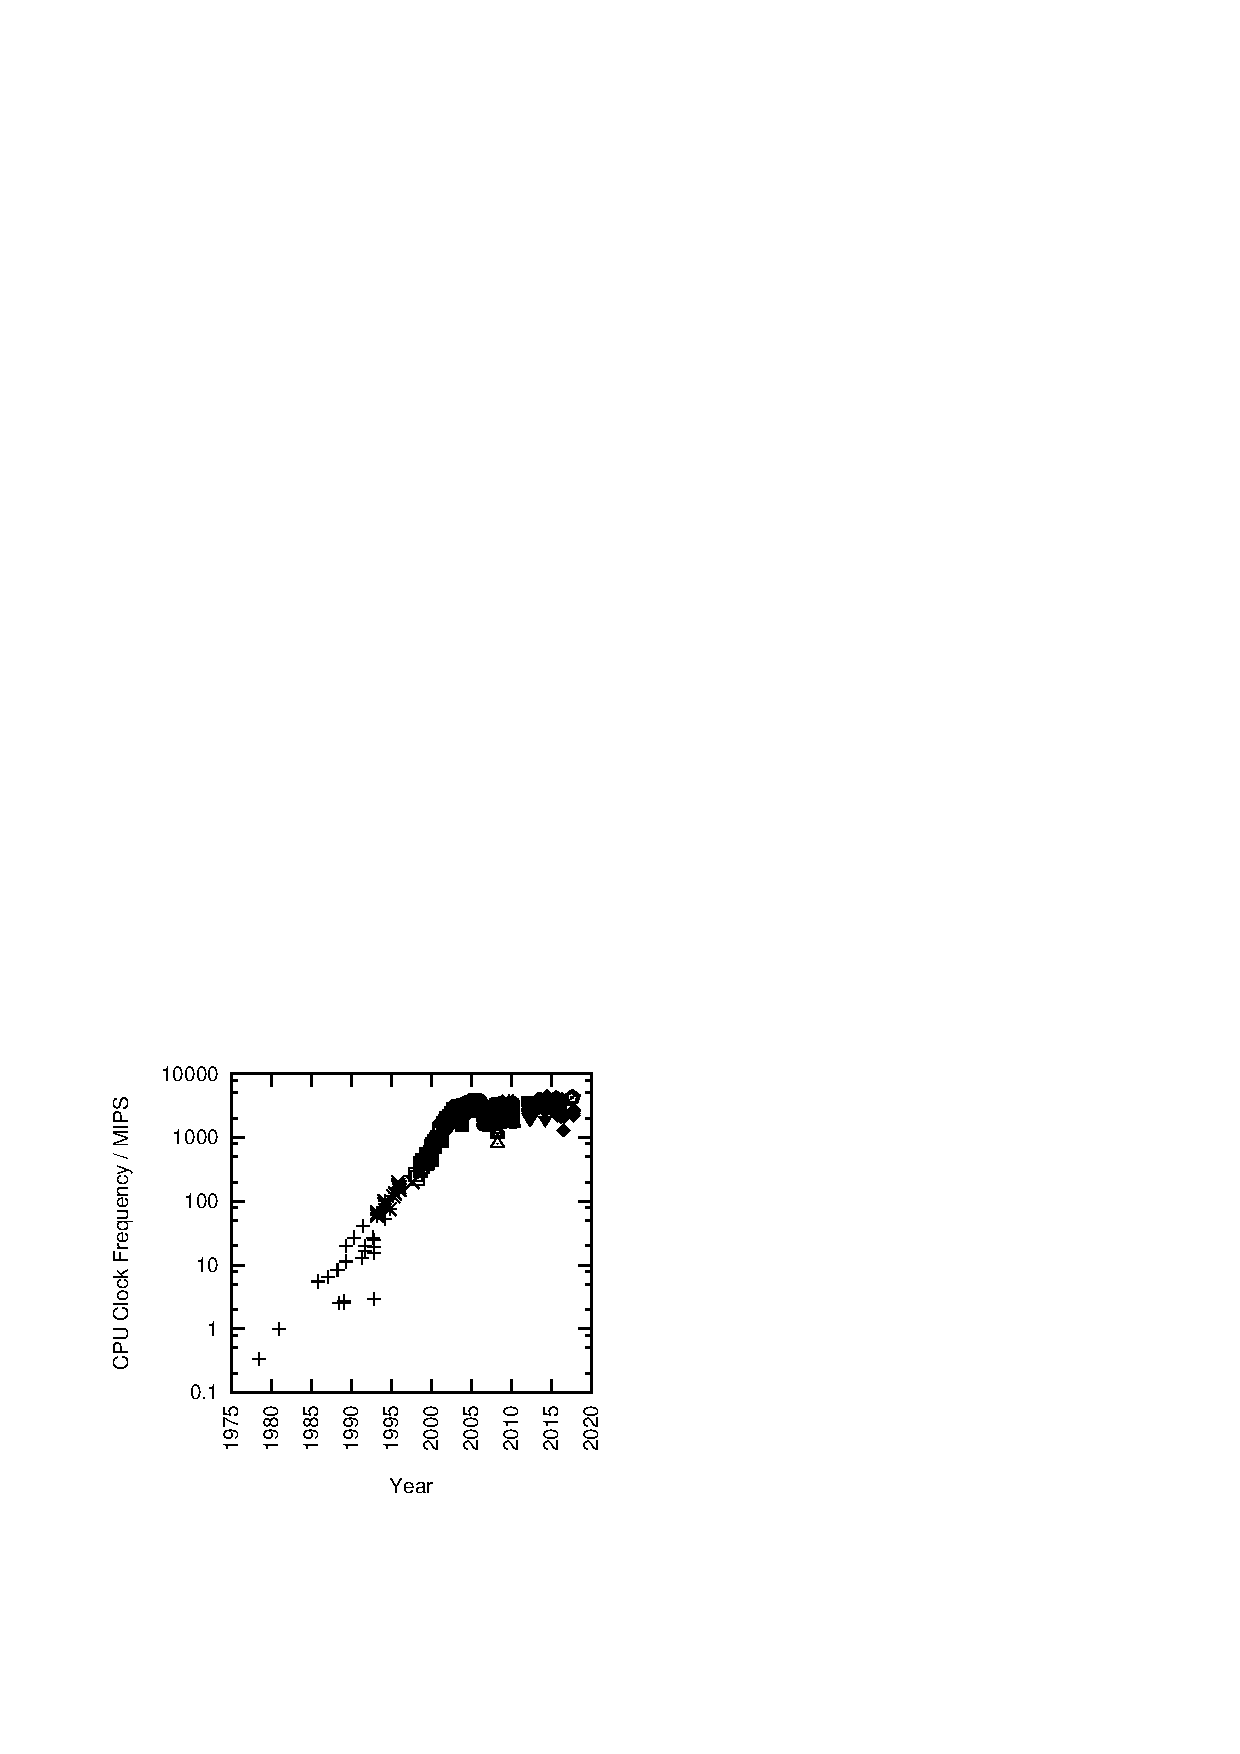
\includegraphics{SMPdesign/clockfreq}}
\caption{MIPS/Clock-Frequency Trend for Intel CPUs}
\label{fig:SMPdesign:Clock-Frequency Trend for Intel CPUs}
\end{figure}

\begin{figure}
\centering
\resizebox{3in}{!}{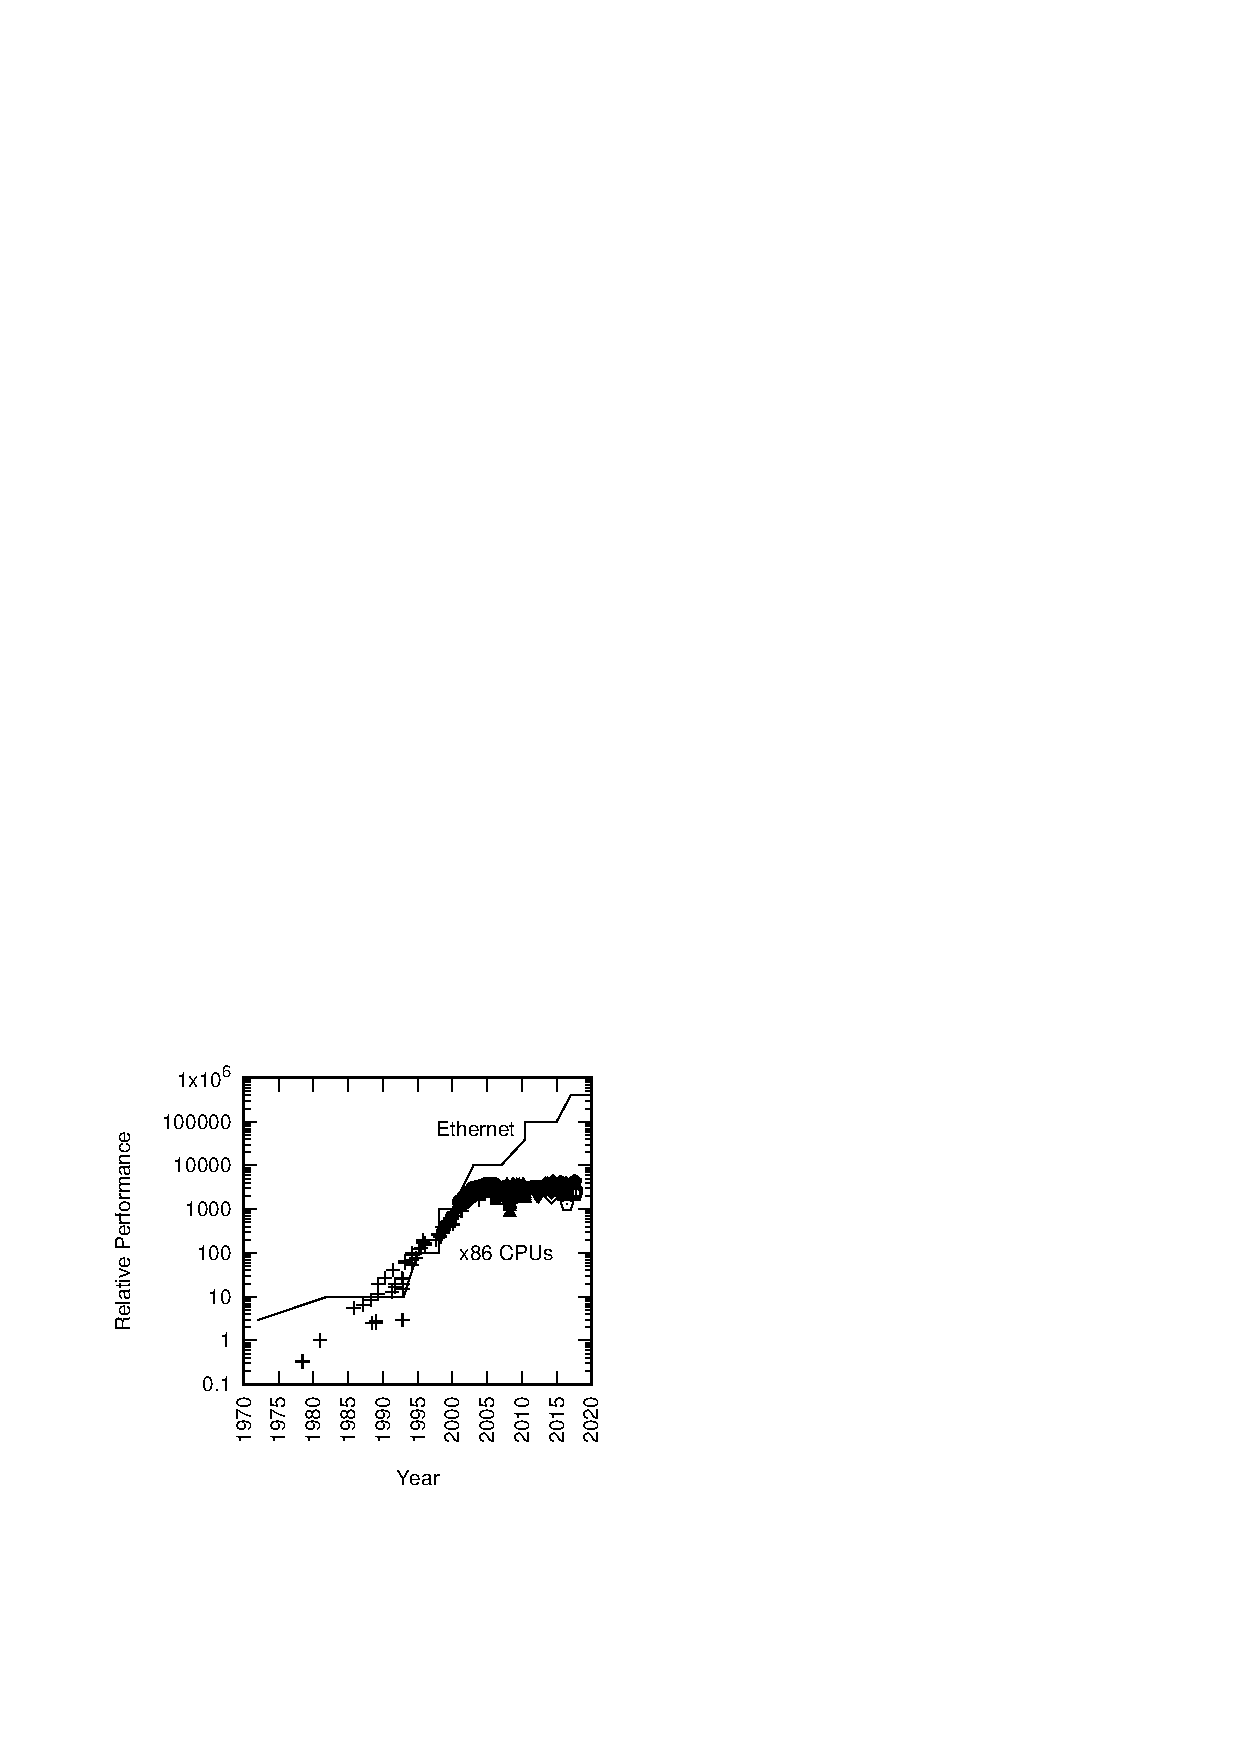
\includegraphics{SMPdesign/CPUvsEnet}}
\caption{Ethernet Bandwidth vs.\@ Intel x86 CPU Performance}
\label{fig:SMPdesign:Ethernet Bandwidth vs. Intel x86 CPU Performance}
\end{figure}

Please note that this does \emph{not} mean that you should code each
and every program in a multi-threaded manner.
Again, if a program runs quickly enough on a single processor,
spare yourself the overhead and complexity of SMP synchronization
primitives.
The simplicity of the hash-table lookup code in
Listing~\ref{lst:SMPdesign:Sequential-Program Hash Table Search}
underscores this point.\footnote{
	The examples in this section are taken from Hart et
	al.~\cite{ThomasEHart2006a}, adapted for clarity
	by gathering related code from multiple files.}
A key point is that speedups due to parallelism are normally
limited to the number of CPUs.
In contrast, speedups due to sequential optimizations, for example,
careful choice of data structure, can be arbitrarily large.

On the other hand, if you are not in this happy situation, read on!

\begin{listing}
\begin{VerbatimL}[commandchars=\\\[\]]
struct hash_table
{
	long nbuckets;
	struct node **buckets;
};

typedef struct node {
	unsigned long key;
	struct node *next;
} node_t;

int hash_search(struct hash_table *h, long key)
{
	struct node *cur;

	cur = h->buckets[key % h->nbuckets];
	while (cur != NULL) {
		if (cur->key >= key) {
			return (cur->key == key);
		}
		cur = cur->next;
	}
	return 0;
}
\end{VerbatimL}
\caption{Sequential-Program Hash Table Search}
\label{lst:SMPdesign:Sequential-Program Hash Table Search}
\end{listing}

% ./test_hash_null.exe 1000 0/100 1 1024 1
% ./test_hash_null.exe: nmilli: 1000 update/total: 0/100 nelements: 1 nbuckets: 1024 nthreads: 1
% ./test_hash_null.exe: avg = 96.2913  max = 98.2337  min = 90.4095  std = 2.95314
% ./test_hash_null.exe: nmilli: 1000 update/total: 0/100 nelements: 1 nbuckets: 1024 nthreads: 1
% ./test_hash_null.exe: avg = 91.5592  max = 97.3315  min = 89.9885  std = 2.88925
% ./test_hash_null.exe: nmilli: 1000 update/total: 0/100 nelements: 1 nbuckets: 1024 nthreads: 1
% ./test_hash_null.exe: avg = 93.3568  max = 106.162  min = 89.8828  std = 6.40418

\subsection{Code Locking}
\label{sec:SMPdesign:Code Locking}

\IXh{Code}{locking} is quite simple due to the fact that is uses only
global locks.\footnote{
	If your program instead has locks in data structures,
	or, in the case of Java, uses classes with synchronized
	instances, you are instead using ``data locking'', described
	in Section~\ref{sec:SMPdesign:Data Locking}.}
It is especially
easy to retrofit an existing program to use code locking in
order to run it on a multiprocessor.
If the program has only a single shared resource, code locking
will even give optimal performance.
However, many of the larger and more complex programs
require much of the execution to
occur in \IXpl{critical section}, which in turn causes code locking
to sharply limits their scalability.

Therefore, you should use code locking on programs that spend
only a small fraction of their execution time in critical sections or
from which only modest scaling is required.
In these cases, code locking will provide a relatively simple
program that is very similar to its sequential counterpart,
as can be seen in
Listing~\ref{lst:SMPdesign:Code-Locking Hash Table Search}.
However, note that the simple return of the comparison in
\co{hash_search()} in
Listing~\ref{lst:SMPdesign:Sequential-Program Hash Table Search}
has now become three statements due to the need to release the
lock before returning.

\begin{listing}
\begin{VerbatimL}[commandchars=\\\[\]]
spinlock_t hash_lock;

struct hash_table
{
	long nbuckets;
	struct node **buckets;
};

typedef struct node {
	unsigned long key;
	struct node *next;
} node_t;

int hash_search(struct hash_table *h, long key)
{
	struct node *cur;
	int retval;

	spin_lock(&hash_lock);
	cur = h->buckets[key % h->nbuckets];
	while (cur != NULL) {
		if (cur->key >= key) {
			retval = (cur->key == key);
			spin_unlock(&hash_lock);
			return retval;
		}
		cur = cur->next;
	}
	spin_unlock(&hash_lock);
	return 0;
}
\end{VerbatimL}
\caption{Code-Locking Hash Table Search}
\label{lst:SMPdesign:Code-Locking Hash Table Search}
\end{listing}

Unfortunately, code locking is particularly prone to ``\IX{lock contention}'',
where multiple CPUs need to acquire the lock concurrently.
SMP programmers who have taken care of groups of small children
(or groups of older people who are acting like children) will immediately
recognize the danger of having only one of something,
as illustrated in Figure~\ref{fig:SMPdesign:Lock Contention}.

% ./test_hash_codelock.exe 1000 0/100 1 1024 1
% ./test_hash_codelock.exe: nmilli: 1000 update/total: 0/100 nelements: 1 nbuckets: 1024 nthreads: 1
% ./test_hash_codelock.exe: avg = 164.115  max = 170.388  min = 161.659  std = 3.21857
% ./test_hash_codelock.exe: nmilli: 1000 update/total: 0/100 nelements: 1 nbuckets: 1024 nthreads: 1
% ./test_hash_codelock.exe: avg = 181.17  max = 198.4  min = 162.459  std = 15.8585
% ./test_hash_codelock.exe: nmilli: 1000 update/total: 0/100 nelements: 1 nbuckets: 1024 nthreads: 1
% ./test_hash_codelock.exe: avg = 167.651  max = 189.014  min = 162.144  std = 10.6819

% ./test_hash_codelock.exe 1000 0/100 1 1024 2
% ./test_hash_codelock.exe: nmilli: 1000 update/total: 0/100 nelements: 1 nbuckets: 1024 nthreads: 2
% ./test_hash_codelock.exe: avg = 378.481  max = 385.971  min = 374.235  std = 4.05934
% ./test_hash_codelock.exe: nmilli: 1000 update/total: 0/100 nelements: 1 nbuckets: 1024 nthreads: 2
% ./test_hash_codelock.exe: avg = 753.414  max = 1015.28  min = 377.734  std = 294.942
% ./test_hash_codelock.exe: nmilli: 1000 update/total: 0/100 nelements: 1 nbuckets: 1024 nthreads: 2
% ./test_hash_codelock.exe: avg = 502.737  max = 980.924  min = 374.406  std = 239.383

One solution to this problem, named ``data locking'', is described
in the next section.

\begin{figure}
\centering
\resizebox{2.5in}{!}{\includegraphics{cartoons/r-2014-Data-one-fighting}}
\caption{Lock Contention}
\ContributedBy{Figure}{fig:SMPdesign:Lock Contention}{Melissa Broussard}
\end{figure}

\subsection{Data Locking}
\label{sec:SMPdesign:Data Locking}

Many data structures may be partitioned,
with each partition of the data structure having its own lock.
Then the \IXpl{critical section} for each part of the data structure
can execute in parallel,
although only one instance of the critical section for a given
part could be executing at a given time.
You should use data locking when contention must
be reduced, and where synchronization overhead is not
limiting speedups.
Data locking reduces contention by distributing the instances
of the overly-large critical section across multiple data structures,
for example, maintaining per-hash-bucket critical sections in a
hash table, as shown in
Listing~\ref{lst:SMPdesign:Data-Locking Hash Table Search}.
The increased scalability again results in a slight increase in complexity
in the form of an additional data structure, the \co{struct bucket}.

\begin{listing}
\begin{VerbatimL}
struct hash_table
{
	long nbuckets;
	struct bucket **buckets;
};

struct bucket {
	spinlock_t bucket_lock;
	node_t *list_head;
};

typedef struct node {
	unsigned long key;
	struct node *next;
} node_t;

int hash_search(struct hash_table *h, long key)
{
	struct bucket *bp;
	struct node *cur;
	int retval;

	bp = h->buckets[key % h->nbuckets];
	spin_lock(&bp->bucket_lock);
	cur = bp->list_head;
	while (cur != NULL) {
		if (cur->key >= key) {
			retval = (cur->key == key);
			spin_unlock(&bp->bucket_lock);
			return retval;
		}
		cur = cur->next;
	}
	spin_unlock(&bp->bucket_lock);
	return 0;
}
\end{VerbatimL}
\caption{Data-Locking Hash Table Search}
\label{lst:SMPdesign:Data-Locking Hash Table Search}
\end{listing}

In contrast with the contentious situation
shown in Figure~\ref{fig:SMPdesign:Lock Contention},
data locking helps promote harmony, as illustrated by
Figure~\ref{fig:SMPdesign:Data Locking}---and in parallel programs,
this \emph{almost} always translates into increased performance and
scalability.
For this reason, data locking was heavily used by Sequent in its
kernels~\cite{Beck85,Inman85,Garg90,Dove90,McKenney92b,McKenney92a,McKenney93}.

\begin{figure}
\centering
\resizebox{2.4in}{!}{\includegraphics{cartoons/r-2014-Data-many-happy}}
\caption{Data Locking}
\ContributedBy{Figure}{fig:SMPdesign:Data Locking}{Melissa Broussard}
\end{figure}

% ./test_hash_spinlock.exe 1000 0/100 1 1024 1
% ./test_hash_spinlock.exe: nmilli: 1000 update/total: 0/100 nelements: 1 nbuckets: 1024 nthreads: 1
% ./test_hash_spinlock.exe: avg = 158.118  max = 162.404  min = 156.199  std = 2.19391
% ./test_hash_spinlock.exe: nmilli: 1000 update/total: 0/100 nelements: 1 nbuckets: 1024 nthreads: 1
% ./test_hash_spinlock.exe: avg = 157.717  max = 162.446  min = 156.415  std = 2.36662
% ./test_hash_spinlock.exe: nmilli: 1000 update/total: 0/100 nelements: 1 nbuckets: 1024 nthreads: 1
% ./test_hash_spinlock.exe: avg = 158.369  max = 164.75  min = 156.501  std = 3.19454

% ./test_hash_spinlock.exe 1000 0/100 1 1024 2
% ./test_hash_spinlock.exe: nmilli: 1000 update/total: 0/100 nelements: 1 nbuckets: 1024 nthreads: 2
% ./test_hash_spinlock.exe: avg = 223.426  max = 422.948  min = 167.858  std = 100.136
% ./test_hash_spinlock.exe: nmilli: 1000 update/total: 0/100 nelements: 1 nbuckets: 1024 nthreads: 2
% ./test_hash_spinlock.exe: avg = 235.462  max = 507.134  min = 167.466  std = 135.836
% ./test_hash_spinlock.exe: nmilli: 1000 update/total: 0/100 nelements: 1 nbuckets: 1024 nthreads: 2
% ./test_hash_spinlock.exe: avg = 305.807  max = 481.685  min = 167.939  std = 132.589

However, as those who have taken care of small children can again attest,
even providing enough to go around is no guarantee of tranquillity.
The analogous situation can arise in SMP programs.
For example, the Linux kernel maintains a cache of files and directories
(called ``dcache'').
Each entry in this cache has its own lock, but the entries corresponding
to the root directory and its direct descendants are much more likely to
be traversed than are more obscure entries.
This can result in many CPUs contending for the locks of these popular
entries, resulting in a situation not unlike that
shown in Figure~\ref{fig:SMPdesign:Data and Skew}.

\begin{figure}
\centering
\resizebox{\twocolumnwidth}{!}{\includegraphics{cartoons/r-2014-Data-many-fighting}}
\caption{Data Locking and Skew}
\ContributedBy{Figure}{fig:SMPdesign:Data and Skew}{Melissa Broussard}
\end{figure}

In many cases, algorithms can be designed to reduce the instance of
data skew, and in some cases eliminate it entirely
(for example, in the Linux kernel's
dcache~\cite{McKenney04a,JonathanCorbet2010dcacheRCU,NeilBrown2015PathnameLookup,NeilBrown2015RCUwalk,NeilBrown2015PathnameSymlinks}).
Data locking is often used for partitionable data structures such as
hash tables, as well as in situations where multiple entities are each
represented by an instance of a given data structure.
The Linux-kernel task list is an example of the latter, each task
structure having its own \co{alloc_lock} and \co{pi_lock}.

A key challenge with data locking on dynamically allocated structures
is ensuring that the structure remains in existence while the lock is
being acquired~\cite{Gamsa99}.
The code in
Listing~\ref{lst:SMPdesign:Data-Locking Hash Table Search}
finesses this challenge by placing the locks in the statically allocated
hash buckets, which are never freed.
However, this trick would not work if the hash table were resizeable,
so that the locks were now dynamically allocated.
In this case, there would need to be some means to prevent the hash
bucket from being freed during the time that its lock was being acquired.

\QuickQuiz{
	What are some ways of preventing a structure from being freed while
	its lock is being acquired?
}\QuickQuizAnswer{
	Here are a few possible solutions to this \emph{existence guarantee}
	problem:

	\begin{enumerate}
	\item	Provide a statically allocated lock that is held while
		the per-structure lock is being acquired, which is an
		example of hierarchical locking (see
		Section~\ref{sec:SMPdesign:Hierarchical Locking}).
		Of course, using a single global lock for this purpose
		can result in unacceptably high levels of lock contention,
		dramatically reducing performance and scalability.
	\item	Provide an array of statically allocated locks, hashing
		the structure's address to select the lock to be acquired,
		as described in Chapter~\ref{chp:Locking}.
		Given a hash function of sufficiently high quality, this
		avoids the scalability limitations of the single global
		lock, but in read-mostly situations, the lock-acquisition
		overhead can result in unacceptably degraded performance.
	\item	Use a garbage collector, in software environments providing
		them, so that a structure cannot be deallocated while being
		referenced.
		This works very well, removing the existence-guarantee
		burden (and much else besides) from the developer's
		shoulders, but imposes the overhead of garbage collection
		on the program.
		Although garbage-collection technology has advanced
		considerably in the past few decades, its overhead
		may be unacceptably high for some applications.
		In addition, some applications require that the developer
		exercise more control over the layout and placement of
		data structures than is permitted by most garbage collected
		environments.
	\item	As a special case of a garbage collector, use a global
		reference counter, or a global array of reference counters.
		These have strengths and limitations similar to those
		called out above for locks.
	\item	Use \emph{hazard pointers}~\cite{MagedMichael04a}, which
		can be thought of as an inside-out reference count.
		Hazard-pointer-based algorithms maintain a per-thread list of
		pointers, so that the appearance of a given pointer on
		any of these lists acts as a reference to the corresponding
		structure.
		Hazard pointers are starting to see significant production use
		(see \cref{sec:defer:Production Uses of Hazard Pointers}).
	\item	Use transactional memory
		(TM)~\cite{Herlihy93a,DBLomet1977SIGSOFT,Shavit95},
		so that each reference and
		modification to the data structure in question is
		performed atomically.
		Although TM has engendered much excitement in recent years,
		and seems likely to be of some use in production software,
		developers should exercise some
		caution~\cite{Blundell2005DebunkTM,Blundell2006TMdeadlock,McKenney2007PLOSTM},
		particularly in performance-critical code.
		In particular, existence guarantees require that the
		transaction covers the full path from a global reference
		to the data elements being updated.
		For more on TM, including ways to overcome some of its
		weaknesses by combining it with other synchronization
		mechanisms, see
		\cref{sec:future:Transactional Memory,sec:future:Hardware Transactional Memory}.
	\item	Use RCU, which can be thought of as an extremely lightweight
		approximation to a garbage collector.
		Updaters are not permitted to free RCU-protected
		data structures that RCU readers might still be referencing.
		RCU is most heavily used for read-mostly data structures,
		and is discussed at length in
		\cref{sec:defer:Read-Copy Update (RCU)}.
	\end{enumerate}

	For more on providing existence guarantees, see
	Chapters~\ref{chp:Locking} and \ref{chp:Deferred Processing}.
}\QuickQuizEnd

\subsection{Data Ownership}
\label{sec:SMPdesign:Data Ownership}

Data ownership partitions a given data structure over the threads
or CPUs, so that each thread/CPU accesses its subset of the data
structure without any synchronization overhead whatsoever.
However, if one thread wishes to access some other thread's data,
the first thread is unable to do so directly.
Instead, the first thread must communicate with the second thread,
so that the second thread performs the operation on behalf of the
first, or, alternatively, migrates the data to the first thread.

Data ownership might seem arcane, but it is used very frequently:
\begin{enumerate}
\item	Any variables accessible by only one CPU or thread
	(such as {\tt auto} variables in C
	and C++) are owned by that CPU or process.
\item	An instance of a user interface owns the corresponding
	user's context.
	It is very common for applications interacting with parallel
	database engines to be written as if they were entirely
	sequential programs.
	Such applications own the user interface and his current
	action.
	Explicit parallelism is thus confined to the
	database engine itself.
\item	Parametric simulations are often trivially parallelized
	by granting each thread ownership of a particular region
	of the parameter space.
	There are also computing frameworks designed for this
	type of problem~\cite{BOINC2008}.
\end{enumerate}

If there is significant sharing, communication between the threads
or CPUs can result in significant complexity and overhead.
Furthermore, if the most-heavily used data happens to be that owned
by a single CPU, that CPU will be a ``hot spot'', sometimes with
results resembling that shown in Figure~\ref{fig:SMPdesign:Data and Skew}.
However, in situations where no sharing is required, data ownership
achieves ideal performance, and with code that can be as simple
as the sequential-program case shown in
Listing~\ref{lst:SMPdesign:Sequential-Program Hash Table Search}.
Such situations are often referred to as ``\IX{embarrassingly
parallel}'', and, in the best case, resemble the situation
previously shown in Figure~\ref{fig:SMPdesign:Data Locking}.

% ./test_hash_null.exe 1000 0/100 1 1024 1
% ./test_hash_null.exe: nmilli: 1000 update/total: 0/100 nelements: 1 nbuckets: 1024 nthreads: 1
% ./test_hash_null.exe: avg = 96.2913  max = 98.2337  min = 90.4095  std = 2.95314
% ./test_hash_null.exe: nmilli: 1000 update/total: 0/100 nelements: 1 nbuckets: 1024 nthreads: 1
% ./test_hash_null.exe: avg = 91.5592  max = 97.3315  min = 89.9885  std = 2.88925
% ./test_hash_null.exe: nmilli: 1000 update/total: 0/100 nelements: 1 nbuckets: 1024 nthreads: 1
% ./test_hash_null.exe: avg = 93.3568  max = 106.162  min = 89.8828  std = 6.40418

% ./test_hash_null.exe 1000 0/100 1 1024 2
% ./test_hash_null.exe: nmilli: 1000 update/total: 0/100 nelements: 1 nbuckets: 1024 nthreads: 2
% ./test_hash_null.exe: avg = 45.4526  max = 46.4281  min = 45.1954  std = 0.487791
% ./test_hash_null.exe: nmilli: 1000 update/total: 0/100 nelements: 1 nbuckets: 1024 nthreads: 2
% ./test_hash_null.exe: avg = 46.0238  max = 49.2861  min = 45.1852  std = 1.63127
% ./test_hash_null.exe: nmilli: 1000 update/total: 0/100 nelements: 1 nbuckets: 1024 nthreads: 2
% ./test_hash_null.exe: avg = 46.6858  max = 52.6278  min = 45.1761  std = 2.97102

Another important instance of data ownership occurs when the data
is read-only, in which case,
all threads can ``own'' it via replication.

Data ownership will be presented in more detail in
Chapter~\ref{chp:Data Ownership}.

\subsection{Locking Granularity and Performance}
\label{sec:SMPdesign:Locking Granularity and Performance}

This section looks at locking granularity and performance from
a mathematical synchronization\-/efficiency viewpoint.
Readers who are uninspired by mathematics might choose to skip
this section.

The approach is to use a crude queueing model for the efficiency of
synchronization mechanism that operate on a single shared global
variable, based on an M/M/1 queue.
M/M/1 queuing models are based on an exponentially distributed
``inter-arrival rate'' $\lambda$ and an exponentially distributed
``service rate'' $\mu$.
The inter-arrival rate $\lambda$ can be thought of as the average
number of synchronization operations per second that the system
would process if the synchronization were free, in other words,
$\lambda$ is an inverse measure of the overhead of each non-synchronization
unit of work.
For example, if each unit of work was a transaction, and if each transaction
took one millisecond to process, excluding synchronization overhead,
then $\lambda$ would be 1,000~transactions per second.

The service rate $\mu$ is defined similarly, but for the average
number of synchronization operations per second that the system
would process if the overhead of each transaction was zero, and
ignoring the fact that CPUs must wait on each other to complete
their synchronization operations, in other words, $\mu$ can be roughly
thought of as the synchronization overhead in absence of contention.
For example, suppose that each transaction's synchronization operation
involves an atomic increment instruction, and that a computer system is
able to do a private-variable atomic increment every 5~nanoseconds on
each CPU
(see \cref{fig:count:Atomic Increment Scalability on x86}).\footnote{
	Of course, if there are 8 CPUs all incrementing the same
	shared variable, then each CPU must wait at least 35~nanoseconds
	for each of the other CPUs to do its increment before consuming
	an additional 5~nanoseconds doing its own increment.
	In fact, the wait will be longer due to the need
	to move the variable from one CPU to another.}
The value of $\mu$ is therefore about 200,000,000 atomic increments
per second.

Of course, the value of $\lambda$ increases as increasing numbers of CPUs
increment a shared variable because each CPU is capable of processing
transactions independently (again, ignoring synchronization):

\begin{equation}
	\lambda = n \lambda_0
\end{equation}

Here, $n$ is the number of CPUs and $\lambda_0$ is the transaction-processing
capability of a single CPU\@.
Note that the expected time for a single CPU to execute a single transaction
in the absence of contention is $1 / \lambda_0$.

Because the CPUs have to ``wait in line'' behind each other to get their
chance to increment the single shared variable, we can use the M/M/1
queueing-model expression for the expected total waiting time:

\begin{equation}
	T = \frac{1}{\mu - \lambda}
\end{equation}

Substituting the above value of $\lambda$:

\begin{equation}
	T = \frac{1}{\mu - n \lambda_0}
\end{equation}

Now, the efficiency is just the ratio of the time required to process
a transaction in absence of synchronization ($1 / \lambda_0$)
to the time required including synchronization ($T + 1 / \lambda_0$):

\begin{equation}
	e = \frac{1 / \lambda_0}{T + 1 / \lambda_0}
\end{equation}

Substituting the above value for $T$ and simplifying:

\begin{equation}
	e = \frac{\frac{\mu}{\lambda_0} - n}{\frac{\mu}{\lambda_0} - (n - 1)}
\end{equation}

But the value of $\mu / \lambda_0$ is just the ratio of the time required
to process the transaction (absent synchronization overhead) to that of
the synchronization overhead itself (absent contention).
If we call this ratio $f$, we have:

\begin{equation}
	e = \frac{f - n}{f - (n - 1)}
\end{equation}

\begin{figure}
\centering
\resizebox{2.5in}{!}{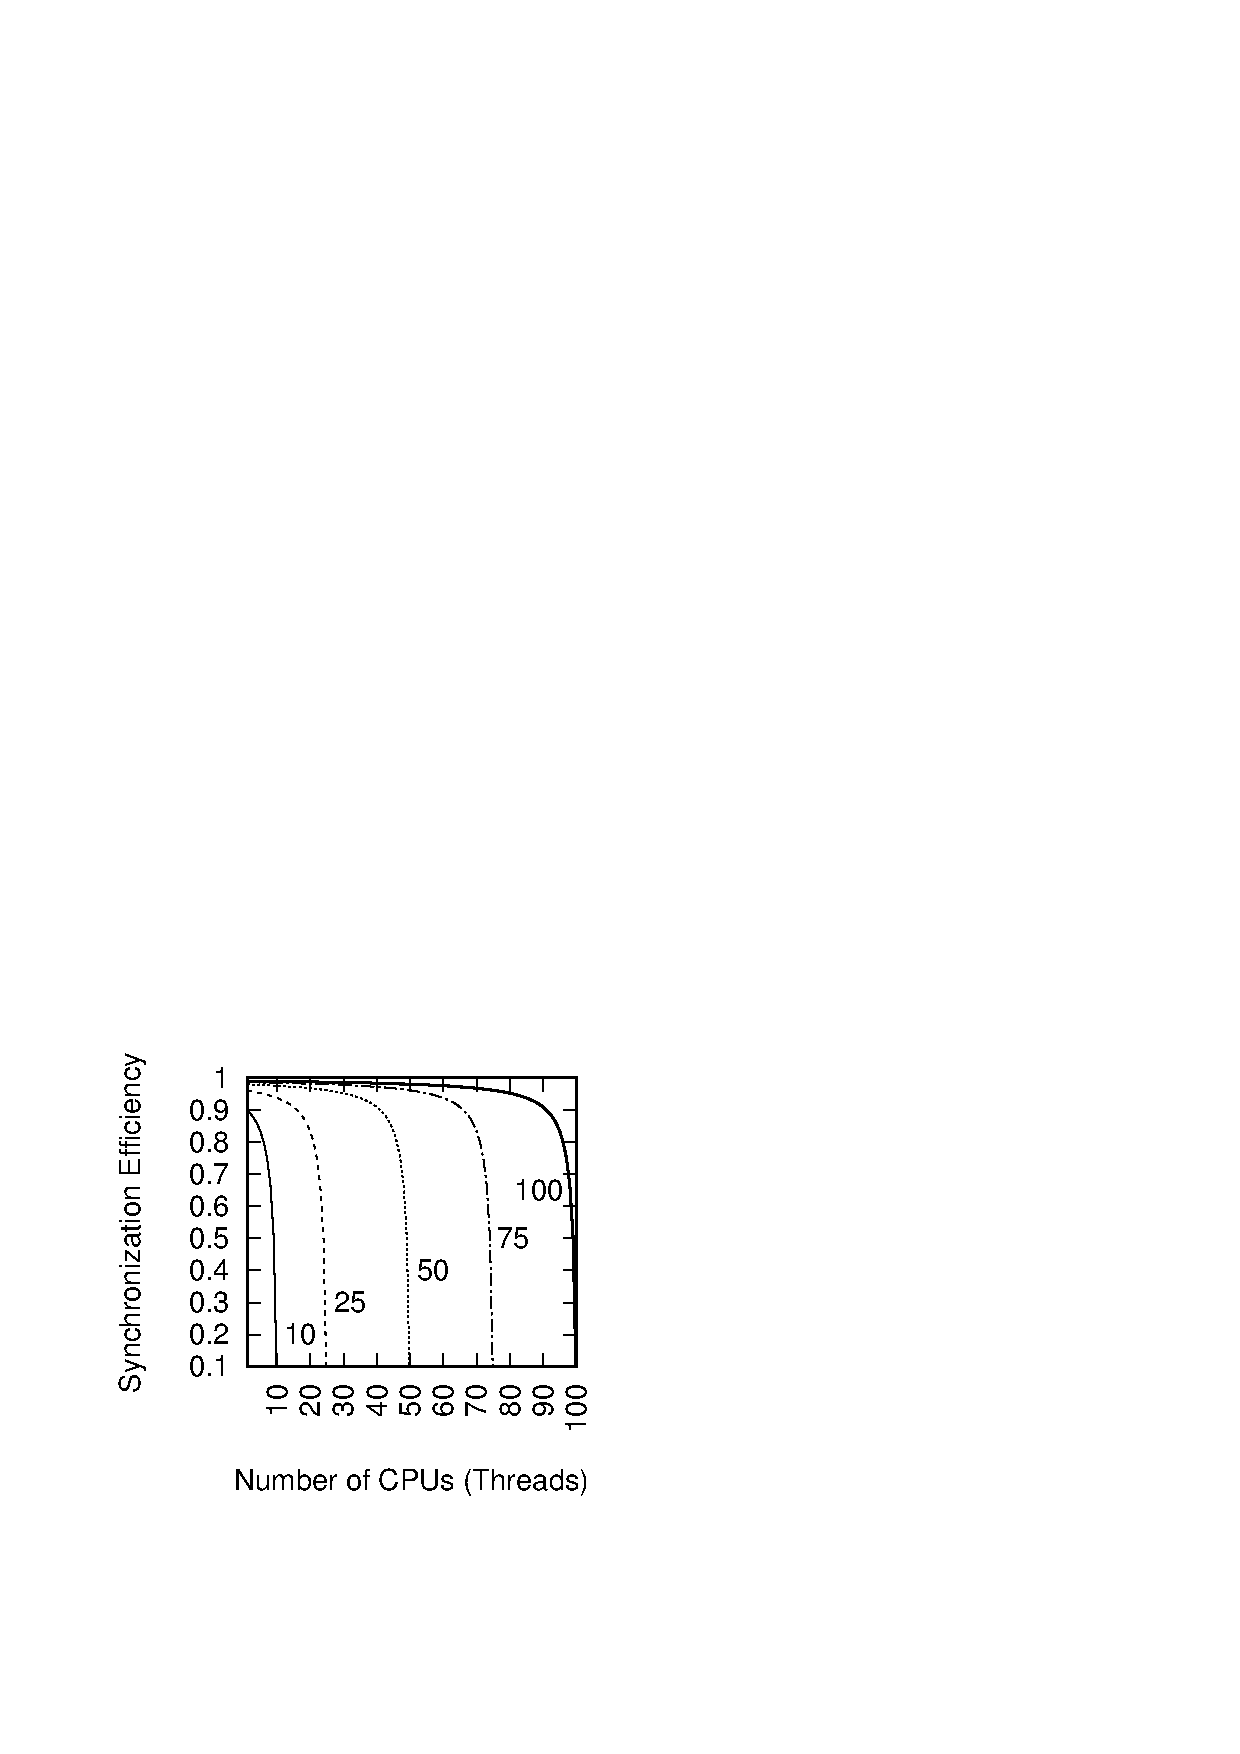
\includegraphics{SMPdesign/synceff}}
\caption{Synchronization Efficiency}
\label{fig:SMPdesign:Synchronization Efficiency}
\end{figure}

Figure~\ref{fig:SMPdesign:Synchronization Efficiency} plots the synchronization
efficiency $e$ as a function of the number of CPUs/threads $n$ for
a few values of the overhead ratio $f$.
For example, again using the 5-nanosecond atomic increment, the $f=10$
line corresponds to each CPU attempting an atomic increment every
50~nanoseconds, and the $f=100$ line corresponds to each CPU attempting
an atomic increment every 500~nanoseconds, which in turn corresponds to
some hundreds (perhaps thousands) of instructions.
Given that each trace drops off sharply with increasing numbers of
CPUs or threads, we can conclude that
synchronization mechanisms based on
atomic manipulation of a single global shared variable will not
scale well if used heavily on current commodity hardware.
This is an abstract mathematical depiction of the forces leading
to the parallel counting algorithms that were discussed in
Chapter~\ref{chp:Counting}.
Your real-world mileage may differ.

Nevertheless, the concept of efficiency is useful, and even in cases
having little or no formal synchronization.
Consider for example a matrix multiply, in which the columns of one
matrix are multiplied (via ``dot product'') by the rows of another,
resulting in an entry in a third matrix.
Because none of these operations conflict, it is possible to partition
the columns of the first matrix among a group of threads, with each thread
computing the corresponding columns of the result matrix.
The threads can therefore operate entirely independently, with no
synchronization overhead whatsoever, as is done in
\path{matmul.c}.
One might therefore expect a perfect efficiency of 1.0.

\begin{figure}
\centering
\resizebox{2.5in}{!}{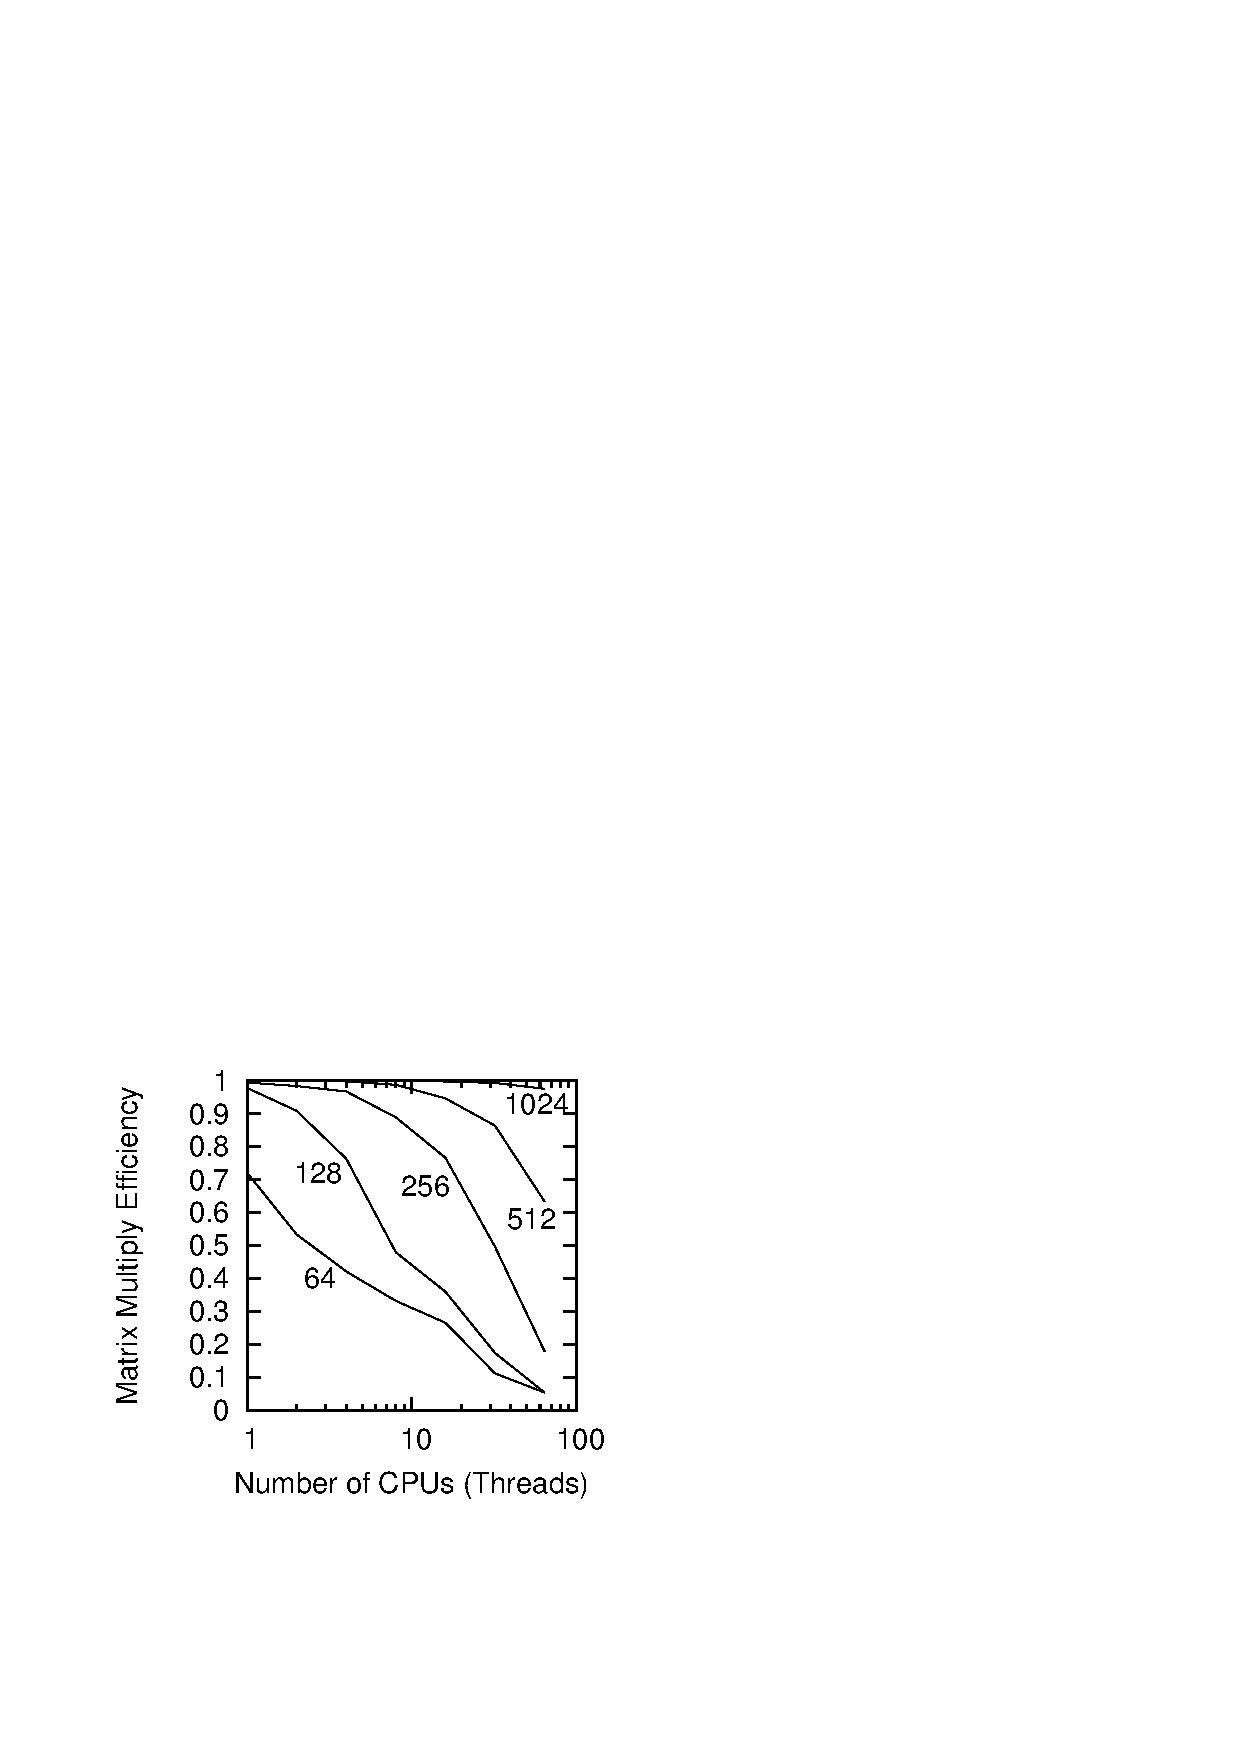
\includegraphics{SMPdesign/matmuleff}}
\caption{Matrix Multiply Efficiency}
\label{fig:SMPdesign:Matrix Multiply Efficiency}
\end{figure}

However,
Figure~\ref{fig:SMPdesign:Matrix Multiply Efficiency}
tells a different story, especially for a 64-by-64 matrix multiply,
which never gets above an efficiency of about 0.3, even when running
single-threaded, and drops sharply as more threads are added.\footnote{
	In contrast to the smooth traces of
	\cref{fig:SMPdesign:Synchronization Efficiency},
	the wide error bars and jagged traces of
	\cref{fig:SMPdesign:Matrix Multiply Efficiency}
	gives evidence of its real-world nature.}
The 128-by-128 matrix does better, but still fails to demonstrate
much performance increase with added threads.
The 256-by-256 matrix does scale reasonably well, but only up to a handful
of CPUs.
The 512-by-512 matrix multiply's efficiency is measurably less
than 1.0 on as few as 10 threads, and even the 1024-by-1024 matrix
multiply deviates noticeably from perfection at a few tens of threads.
Nevertheless, this figure clearly demonstrates the performance and
scalability benefits of batching: If you must incur synchronization
overhead, you may as well get your money's worth.

\QuickQuiz{
	How can a single-threaded 64-by-64 matrix multiple possibly
	have an efficiency of less than 1.0?
	Shouldn't all of the traces in
	Figure~\ref{fig:SMPdesign:Matrix Multiply Efficiency}
	have efficiency of exactly 1.0 when running on one thread?
}\QuickQuizAnswer{
	The \path{matmul.c} program creates the specified number of
	worker threads, so even the single-worker-thread case incurs
	thread-creation overhead.
	Making the changes required to optimize away thread-creation
	overhead in the single-worker-thread case is left as an
	exercise to the reader.
}\QuickQuizEnd

Given these inefficiencies,
it is worthwhile to look into more-scalable approaches
such as the data locking described in
Section~\ref{sec:SMPdesign:Data Locking}
or the parallel-fastpath approach discussed in the next section.

\QuickQuiz{
	How are data-parallel techniques going to help with matrix
	multiply?
	It is \emph{already} data parallel!!!
}\QuickQuizAnswer{
	I am glad that you are paying attention!
	This example serves to show that although data parallelism can
	be a very good thing, it is not some magic wand that automatically
	wards off any and all sources of inefficiency.
	Linear scaling at full performance, even to ``only'' 64 threads,
	requires care at all phases of design and implementation.

	In particular, you need to pay careful attention to the
	size of the partitions.
	For example, if you split a 64-by-64 matrix multiply across
	64 threads, each thread gets only 64 floating-point multiplies.
	The cost of a floating-point multiply is minuscule compared to
	the overhead of thread creation, and cache-miss overhead
	also plays a role in spoiling the theoretically perfect scalability
	(and also in making the traces so jagged).
	The full 448~hardware threads would require a matrix with
	hundreds of thousands of rows and columns to attain good
	scalability, but by that point GPGPUs become quite attractive,
	especially from a price/performance viewpoint.

	Moral: If you have a parallel program with variable input,
	always include a check for the input size being too small to
	be worth parallelizing.
	And when it is not helpful to parallelize, it is not helpful
	to incur the overhead required to spawn a thread, now is it?
}\QuickQuizEnd

\section{Parallel Fastpath}
\label{sec:SMPdesign:Parallel Fastpath}
%
\epigraph{There are two ways of meeting difficulties: You alter the
	  difficulties, or you alter yourself to meet them.}
	 {\emph{Phyllis Bottome}}

Fine-grained (and therefore \emph{usually} higher-performance)
designs are typically more complex than are coarser-grained designs.
In many cases, most of the overhead is incurred by a small fraction
of the code~\cite{Knuth73}.
So why not focus effort on that small fraction?

This is the idea behind the parallel-fastpath design pattern, to aggressively
parallelize the common-case code path without incurring the complexity
that would be required to aggressively parallelize the entire algorithm.
You must understand not only the specific algorithm you wish
to parallelize, but also the workload that the algorithm will
be subjected to.
Great creativity and design effort is often required to construct
a parallel fastpath.

Parallel fastpath combines different patterns (one for the
fastpath, one elsewhere) and is therefore a template pattern.
The following instances of parallel
fastpath occur often enough to warrant their own patterns,
as depicted in Figure~\ref{fig:SMPdesign:Parallel-Fastpath Design Patterns}:

\begin{figure}
\centering
\resizebox{2.3in}{!}{\includegraphics{SMPdesign/ParallelFastpath}}
% \includegraphics{SMPdesign/ParallelFastpath}
\caption{Parallel-Fastpath Design Patterns}
\label{fig:SMPdesign:Parallel-Fastpath Design Patterns}
\end{figure}

\begin{enumerate}
\item	Reader/Writer Locking
	(described below in Section~\ref{sec:SMPdesign:Reader/Writer Locking}).
\item	Read-copy update (RCU), which may be used as a high-performance
	replacement for reader/writer locking, is introduced in
	Section~\ref{sec:defer:Read-Copy Update (RCU)}.
	Other alternatives include hazard pointers
	(\cref{sec:defer:Hazard Pointers})
	and sequence locking (\cref{sec:defer:Sequence Locks}).
	These alternatives will not be discussed further in this chapter.
\item   Hierarchical Locking~(\cite{McKenney95b}), which is touched upon
	in Section~\ref{sec:SMPdesign:Hierarchical Locking}.
\item	Resource Allocator Caches~(\cite{McKenney95b,McKenney93}).
	See Section~\ref{sec:SMPdesign:Resource Allocator Caches}
	for more detail.
\end{enumerate}

\subsection{Reader/Writer Locking}
\label{sec:SMPdesign:Reader/Writer Locking}

If synchronization overhead is negligible (for example, if the program
uses coarse-grained parallelism with large \IXpl{critical section}), and if
only a small fraction of the critical sections modify data, then allowing
multiple readers to proceed in parallel can greatly increase scalability.
Writers exclude both readers and each other.
There are many implementations of reader-writer locking, including
the POSIX implementation described in
Section~\ref{sec:toolsoftrade:POSIX Reader-Writer Locking}.
Listing~\ref{lst:SMPdesign:Reader-Writer-Locking Hash Table Search}
shows how the hash search might be implemented using reader-writer locking.

\begin{listing}
\begin{VerbatimL}[commandchars=\\\[\]]
rwlock_t hash_lock;

struct hash_table
{
	long nbuckets;
	struct node **buckets;
};

typedef struct node {
	unsigned long key;
	struct node *next;
} node_t;

int hash_search(struct hash_table *h, long key)
{
	struct node *cur;
	int retval;

	read_lock(&hash_lock);
	cur = h->buckets[key % h->nbuckets];
	while (cur != NULL) {
		if (cur->key >= key) {
			retval = (cur->key == key);
			read_unlock(&hash_lock);
			return retval;
		}
		cur = cur->next;
	}
	read_unlock(&hash_lock);
	return 0;
}
\end{VerbatimL}
\caption{Reader-Writer-Locking Hash Table Search}
\label{lst:SMPdesign:Reader-Writer-Locking Hash Table Search}
\end{listing}

Reader/writer locking is a simple instance of asymmetric locking.
Snaman~\cite{Snaman87} describes a more ornate six-mode
asymmetric locking design used in several clustered systems.
Locking in general and reader-writer locking in particular is described
extensively in
Chapter~\ref{chp:Locking}.

\subsection{Hierarchical Locking}
\label{sec:SMPdesign:Hierarchical Locking}

The idea behind hierarchical locking is to have a coarse-grained lock
that is held only long enough to work out which fine-grained lock
to acquire.
Listing~\ref{lst:SMPdesign:Hierarchical-Locking Hash Table Search}
shows how our hash-table search might be adapted to do hierarchical
locking, but also shows the great weakness of this approach:
we have paid the overhead of acquiring a second lock, but we only
hold it for a short time.
In this case, the simpler data-locking approach would be simpler
and likely perform better.

\begin{listing}
\begin{fcvlabel}[ln:SMPdesign:Hierarchical-Locking Hash Table Search]
\begin{VerbatimL}[commandchars=\\\[\]]
struct hash_table
{
	long nbuckets;
	struct bucket **buckets;
};

struct bucket {
	spinlock_t bucket_lock;
	node_t *list_head;
};

typedef struct node {
	spinlock_t node_lock;
	unsigned long key;
	struct node *next;
} node_t;

int hash_search(struct hash_table *h, long key)
{
	struct bucket *bp;
	struct node *cur;
	int retval;

	bp = h->buckets[key % h->nbuckets];
	spin_lock(&bp->bucket_lock);
	cur = bp->list_head;
	while (cur != NULL) {
		if (cur->key >= key) {
			spin_lock(&cur->node_lock);
			spin_unlock(&bp->bucket_lock);
			retval = (cur->key == key);\lnlbl[retval]
			spin_unlock(&cur->node_lock);
			return retval;
		}
		cur = cur->next;
	}
	spin_unlock(&bp->bucket_lock);
	return 0;
}
\end{VerbatimL}
\end{fcvlabel}
\caption{Hierarchical-Locking Hash Table Search}
\label{lst:SMPdesign:Hierarchical-Locking Hash Table Search}
\end{listing}

\QuickQuiz{
	In what situation would hierarchical locking work well?
}\QuickQuizAnswer{
	If the comparison on
        line~\ref{ln:SMPdesign:Hierarchical-Locking Hash Table Search:retval} of
	Listing~\ref{lst:SMPdesign:Hierarchical-Locking Hash Table Search}
	were replaced by a much heavier-weight operation,
	then releasing \co{bp->bucket_lock} \emph{might} reduce lock
	contention enough to outweigh the overhead of the extra
	acquisition and release of \co{cur->node_lock}.
}\QuickQuizEnd

\subsection{Resource Allocator Caches}
\label{sec:SMPdesign:Resource Allocator Caches}

This section presents a simplified schematic of a parallel fixed-block-size
memory allocator.
More detailed descriptions may be found in the
literature~\cite{McKenney92a,McKenney93,Bonwick01slab,McKenney01e,JasonEvans2011jemalloc,ChrisKennelly2020tcmalloc}
or in the Linux kernel~\cite{Torvalds2.6kernel}.

\subsubsection{Parallel Resource Allocation Problem}

The basic problem facing a parallel memory allocator is the tension
between the need to provide extremely fast memory allocation and
freeing in the common case and the need to efficiently distribute
memory in face of unfavorable allocation and freeing patterns.

To see this tension, consider a straightforward application of
data ownership to this problem---simply carve up memory so that
each CPU owns its share.
For example, suppose that a system with 12~CPUs has 64~gigabytes
of memory, for example, the laptop I am using right now.
We could simply assign each CPU a five-gigabyte region of memory,
and allow each CPU to allocate from its own region, without the need
for locking and its complexities and overheads.
Unfortunately, this scheme fails when CPU~0 only allocates memory and
CPU~1 only frees it, as happens in simple producer-consumer workloads.

The other extreme, \IXh{code}{locking}, suffers from excessive
\IX{lock contention}
and overhead~\cite{McKenney93}.

\subsubsection{Parallel Fastpath for Resource Allocation}
\label{sec:SMPdesign:Parallel Fastpath for Resource Allocation}

The commonly used solution uses parallel fastpath with each CPU
owning a modest cache of blocks, and with a large code-locked
shared pool for additional blocks.
To prevent any given CPU from monopolizing the memory blocks,
we place a limit on the number of blocks that can be in each CPU's
cache.
In a two-CPU system, the flow of memory blocks will be as shown
in Figure~\ref{fig:SMPdesign:Allocator Cache Schematic}:
when a given CPU is trying to free a block when its pool is full,
it sends blocks to the global pool, and, similarly, when that CPU
is trying to allocate a block when its pool is empty, it retrieves
blocks from the global pool.

\begin{figure}
\centering
\resizebox{3in}{!}{\includegraphics{SMPdesign/allocatorcache}}
\caption{Allocator Cache Schematic}
\label{fig:SMPdesign:Allocator Cache Schematic}
\end{figure}

\subsubsection{Data Structures}

The actual data structures for a ``toy'' implementation of allocator
caches are shown in
Listing~\ref{lst:SMPdesign:Allocator-Cache Data Structures}.
The ``Global Pool'' of Figure~\ref{fig:SMPdesign:Allocator Cache Schematic}
is implemented by \co{globalmem} of type \co{struct globalmempool},
and the two CPU pools by the per-thread variable \co{perthreadmem} of
type \co{struct perthreadmempool}.
Both of these data structures have arrays of pointers to blocks
in their \co{pool} fields, which are filled from index zero upwards.
Thus, if \co{globalmem.pool[3]} is \co{NULL}, then the remainder of
the array from index 4 up must also be \co{NULL}.
The \co{cur} fields contain the index of the highest-numbered full
element of the \co{pool} array, or $-1$ if all elements are empty.
All elements from \co{globalmem.pool[0]} through
\co{globalmem.pool[globalmem.cur]} must be full, and all the rest
must be empty.\footnote{
	Both pool sizes (\co{TARGET_POOL_SIZE} and
	\co{GLOBAL_POOL_SIZE}) are unrealistically small, but this small
	size makes it easier to single-step the program in order to get
	a feel for its operation.}

\begin{listing}
\input{CodeSamples/SMPdesign/smpalloc@data_struct.fcv}
\caption{Allocator-Cache Data Structures}
\label{lst:SMPdesign:Allocator-Cache Data Structures}
\end{listing}

The operation of the pool data structures is illustrated by
Figure~\ref{fig:SMPdesign:Allocator Pool Schematic},
with the six boxes representing the array of pointers making up
the \co{pool} field, and the number preceding them representing
the \co{cur} field.
The shaded boxes represent non-\co{NULL} pointers, while the empty
boxes represent \co{NULL} pointers.
An important, though potentially confusing, invariant of this
data structure is that the \co{cur} field is always one
smaller than the number of non-\co{NULL} pointers.

\begin{figure}
\centering
\resizebox{2.6in}{!}{\includegraphics{SMPdesign/AllocatorPool}}
\caption{Allocator Pool Schematic}
\label{fig:SMPdesign:Allocator Pool Schematic}
\end{figure}

\subsubsection{Allocation Function}

\begin{fcvref}[ln:SMPdesign:smpalloc:alloc]
The allocation function \co{memblock_alloc()} may be seen in
Listing~\ref{lst:SMPdesign:Allocator-Cache Allocator Function}.
Line~\lnref{pick} picks up the current thread's per-thread pool,
and line~\lnref{chk:empty} checks to see if it is empty.

If so, \clnrefrange{ack}{rel} attempt to refill it
from the global pool
under the spinlock acquired on line~\lnref{ack} and released on line~\lnref{rel}.
\Clnrefrange{loop:b}{loop:e} move blocks from the global
to the per-thread pool until
either the local pool reaches its target size (half full) or
the global pool is exhausted, and line~\lnref{set} sets the per-thread pool's
count to the proper value.

In either case, line~\lnref{chk:notempty} checks for the per-thread
pool still being
empty, and if not, \clnrefrange{rem:b}{rem:e} remove a block and return it.
Otherwise, line~\lnref{ret:NULL} tells the sad tale of memory exhaustion.
\end{fcvref}

\begin{listing}
\input{CodeSamples/SMPdesign/smpalloc@alloc.fcv}
\caption{Allocator-Cache Allocator Function}
\label{lst:SMPdesign:Allocator-Cache Allocator Function}
\end{listing}

\subsubsection{Free Function}

\begin{fcvref}[ln:SMPdesign:smpalloc:free]
Listing~\ref{lst:SMPdesign:Allocator-Cache Free Function} shows
the memory-block free function.
Line~\lnref{get} gets a pointer to this thread's pool, and
line~\lnref{chk:full} checks to see if this per-thread pool is full.

If so, \clnrefrange{acq}{empty:e} empty half of the per-thread pool
into the global pool,
with lines~\lnref{acq} and~\lnref{rel} acquiring and releasing the spinlock.
\Clnrefrange{loop:b}{loop:e} implement the loop moving blocks
from the local to the
global pool, and line~\lnref{set} sets the per-thread pool's count to the proper
value.

In either case, line~\lnref{place} then places the newly freed block into the
per-thread pool.
\end{fcvref}

\begin{listing}
\input{CodeSamples/SMPdesign/smpalloc@free.fcv}
\caption{Allocator-Cache Free Function}
\label{lst:SMPdesign:Allocator-Cache Free Function}
\end{listing}

\QuickQuiz{
	Doesn't this resource-allocator design resemble that of
	the approximate limit counters covered in
	Section~\ref{sec:count:Approximate Limit Counters}?
}\QuickQuizAnswer{
	Indeed it does!
	We are used to thinking of allocating and freeing memory,
	but the algorithms in
	Section~\ref{sec:count:Approximate Limit Counters}
	are taking very similar actions to allocate and free
	``count''.
}\QuickQuizEnd

\subsubsection{Performance}

Rough performance results\footnote{
	This data was not collected in a statistically meaningful way,
	and therefore should be viewed with great skepticism and suspicion.
	Good data-collection and -reduction practice is discussed
	in Chapter~\ref{chp:Validation}.
	That said, repeated runs gave similar results, and these results
	match more careful evaluations of similar algorithms.}
are shown in
Figure~\ref{fig:SMPdesign:Allocator Cache Performance},
running on a dual-core Intel x86 running at 1\,GHz (4300 bogomips per CPU)
with at most six blocks allowed in each CPU's cache.
In this micro-benchmark,
each thread repeatedly allocates a group of blocks and then frees all
the blocks in that group, with
the number of blocks in the group being the ``allocation run length''
displayed on the x-axis.
The y-axis shows the number of successful allocation/free pairs per
microsecond---failed allocations are not counted.
The ``X''s are from a two-thread run, while the ``+''s are from a
single-threaded run.

\begin{figure}
\centering
\resizebox{2.5in}{!}{\includegraphics{SMPdesign/smpalloc}}
\caption{Allocator Cache Performance}
\label{fig:SMPdesign:Allocator Cache Performance}
\end{figure}

Note that run lengths up to six scale linearly and give excellent performance,
while run lengths greater than six show poor performance and almost always
also show \emph{negative} scaling.
It is therefore quite important to size \co{TARGET_POOL_SIZE}
sufficiently large,
which fortunately is usually quite easy to do in actual
practice~\cite{McKenney01e}, especially given today's large memories.
For example, in most systems, it is quite reasonable to set
\co{TARGET_POOL_SIZE} to 100, in which case allocations and frees
are guaranteed to be confined to per-thread pools at least 99\,\% of
the time.

As can be seen from the figure, the situations where the common-case
data-ownership applies (run lengths up to six) provide greatly improved
performance compared to the cases where locks must be acquired.
Avoiding synchronization in the common case will be a recurring theme through
this book.

\QuickQuizSeries{%
\QuickQuizB{
	In Figure~\ref{fig:SMPdesign:Allocator Cache Performance},
	there is a pattern of performance rising with increasing run
	length in groups of three samples, for example, for run lengths
	10, 11, and 12.
	Why?
}\QuickQuizAnswerB{
	This is due to the per-CPU target value being three.
	A run length of 12 must acquire the global-pool lock twice,
	while a run length of 13 must acquire the global-pool lock
	three times.
}\QuickQuizEndB
%
\QuickQuizE{
	Allocation failures were observed in the two-thread
	tests at run lengths of 19 and greater.
	Given the global-pool size of 40 and the per-thread target
	pool size $s$ of three, number of threads $n$ equal to two,
	and assuming that the per-thread pools are initially
	empty with none of the memory in use, what is the smallest allocation
	run length $m$ at which failures can occur?
	(Recall that each thread repeatedly allocates $m$ block of memory,
	and then frees the $m$ blocks of memory.)
	Alternatively, given $n$ threads each with pool size $s$, and
	where each thread repeatedly first allocates $m$ blocks of memory
	and then frees those $m$ blocks, how large must the global pool
	size be?
	\emph{Note:} Obtaining the correct answer will require you to
	examine the \path{smpalloc.c} source code, and very likely
	single-step it as well.
	You have been warned!
}\QuickQuizAnswerE{
	This solution is adapted from one put forward by Alexey Roytman.
	It is based on the following definitions:

	\begin{description}
	\item[$g$]	Number of blocks globally available.
	\item[$i$]	Number of blocks left in the initializing thread's
			per-thread pool.
			(This is one reason you needed to look at the code!)
	\item[$m$]	Allocation/free run length.
	\item[$n$]	Number of threads, excluding the initialization thread.
	\item[$p$]	Per-thread maximum block consumption, including
			both the blocks actually allocated and the blocks
			remaining in the per-thread pool.
	\end{description}

	The values $g$, $m$, and $n$ are given.
	The value for $p$ is $m$ rounded up to the next multiple of $s$,
	as follows:

	\begin{equation}
		p = s \left \lceil \frac{m}{s} \right \rceil
	\label{sec:SMPdesign:p}
	\end{equation}

	The value for $i$ is as follows:

	\begin{equation}
		i = \left \{
			\begin{array}{l}
				g \pmod{2 s} = 0: 2 s \\
				g \pmod{2 s} \ne 0: g \pmod{2 s}
			\end{array}
		    \right .
	\label{sec:SMPdesign:i}
	\end{equation}

	\begin{figure}
	\centering
	\resizebox{3in}{!}{\includegraphics{SMPdesign/smpalloclim}}
	\caption{Allocator Cache Run-Length Analysis}
	\label{fig:SMPdesign:Allocator Cache Run-Length Analysis}
	\end{figure}

	The relationships between these quantities are shown in
	Figure~\ref{fig:SMPdesign:Allocator Cache Run-Length Analysis}.
	The global pool is shown on the top of this figure, and
	the ``extra'' initializer thread's per-thread pool and
	per-thread allocations are the left-most pair of boxes.
	The initializer thread has no blocks allocated, but has
	$i$ blocks stranded in its per-thread pool.
	The rightmost two pairs of boxes are the per-thread pools and
	per-thread allocations of threads holding the maximum possible
	number of blocks, while the second-from-left pair of boxes
	represents the thread currently trying to allocate.

	The total number of blocks is $g$, and adding up the per-thread
	allocations and per-thread pools, we see that the global pool
	contains $g-i-p(n-1)$ blocks.
	If the allocating thread is to be successful, it needs at least
	$m$ blocks in the global pool, in other words:

	\begin{equation}
		g - i - p(n - 1) \ge m
	\label{sec:SMPdesign:g-vs-m}
	\end{equation}

	The question has $g=40$, $s=3$, and $n=2$.
	Equation~\ref{sec:SMPdesign:i} gives $i=4$, and
	Equation~\ref{sec:SMPdesign:p} gives $p=18$ for $m=18$
	and $p=21$ for $m=19$.
	Plugging these into Equation~\ref{sec:SMPdesign:g-vs-m}
	shows that $m=18$ will not overflow, but that $m=19$ might
	well do so.

	The presence of $i$ could be considered to be a bug.
	After all, why allocate memory only to have it stranded in
	the initialization thread's cache?
	One way of fixing this would be to provide a \co{memblock_flush()}
	function that flushed the current thread's pool into the
	global pool.
	The initialization thread could then invoke this function
	after freeing all of the blocks.
}\QuickQuizEndE
}

\subsubsection{Real-World Design}

The toy parallel resource allocator was quite simple, but real-world
designs expand on this approach in a number of ways.

First, real-world allocators are required to handle a wide range
of allocation sizes, as opposed to the single size shown in this
toy example.
One popular way to do this is to offer a fixed set of sizes, spaced
so as to balance external and internal fragmentation, such as in
the late-1980s BSD memory allocator~\cite{McKusick88}.
Doing this would mean that the ``globalmem'' variable would need
to be replicated on a per-size basis, and that the associated
lock would similarly be replicated, resulting in \IXh{data}{locking}
rather than the toy program's code locking.

Second, production-quality systems must be able to repurpose memory,
meaning that they must be able to coalesce blocks into larger structures,
such as pages~\cite{McKenney93}.
This coalescing will also need to be protected by a lock, which again
could be replicated on a per-size basis.

Third, coalesced memory must be returned to the underlying memory
system, and pages of memory must also be allocated from the underlying
memory system.
The locking required at this level will depend on that of the underlying
memory system, but could well be code locking.
Code locking can often be tolerated at this level, because this
level is so infrequently reached in well-designed systems~\cite{McKenney01e}.

Despite this real-world design's greater complexity, the underlying
idea is the same---repeated application of parallel fastpath,
as shown in
Table~\ref{fig:app:questions:Schematic of Real-World Parallel Allocator}.

\begin{table}
\rowcolors{1}{}{lightgray}
\small
\centering
\renewcommand*{\arraystretch}{1.25}
\begin{tabularx}{\twocolumnwidth}{ll>{\raggedright\arraybackslash}X}
\toprule
Level	& Locking & Purpose \\
\midrule
Per-thread pool	  & Data ownership & High-speed allocation \\
Global block pool & Data locking   & Distributing blocks among threads \\
Coalescing	  & Data locking   & Combining blocks into pages \\
System memory	  & Code locking   & Memory from/to system \\
\bottomrule
\end{tabularx}
\caption{Schematic of Real-World Parallel Allocator}
\label{fig:app:questions:Schematic of Real-World Parallel Allocator}
\end{table}

% beyond.tex

\section{Beyond Partitioning}
\label{sec:SMPdesign:Beyond Partitioning}
\OriginallyPublished{Section}{sec:SMPdesign:Beyond Partitioning}{Retrofitted Parallelism Considered Grossly Sub-Optimal}{4\textsuperscript{th} USENIX Workshop on Hot Topics on Parallelism}{PaulEMcKenney2012HOTPARsuboptimal}

This chapter has discussed how data partitioning can be used to design
simple linearly scalable parallel programs.
Section~\ref{sec:SMPdesign:Data Ownership} hinted at the possibilities
of data replication, which will be used to great effect in
Section~\ref{sec:defer:Read-Copy Update (RCU)}.

The main goal of applying partitioning and replication is to achieve
linear speedups, in other words, to ensure that the total amount of
work required does not increase significantly as the number of CPUs
or threads increases.
A problem that can be solved via partitioning and/or replication,
resulting in linear speedups, is \emph{embarrassingly parallel}.
But can we do better?

To answer this question, let us examine the solution of
labyrinths and mazes.
Of course, labyrinths and mazes have been objects of fascination for
millennia~\cite{WikipediaLabyrinth},
so it should come as no surprise that they are generated and solved
using computers, including biological
computers~\cite{AndrewAdamatzky2011SlimeMold},
GPGPUs~\cite{ChristerEricson2008GPUMaze}, and even
discrete hardware~\cite{MIT:TRMag:MemristorMazes}.
Parallel solution of mazes is sometimes used as a class project in
universities~\cite{ETHZurich:FS2011maze,UMD:CMSC433maze} and
as a vehicle to demonstrate the benefits of parallel-programming
frameworks~\cite{RonFosner2010maze}.

Common advice is to use a parallel work-queue algorithm
(PWQ)~\cite{ETHZurich:FS2011maze,RonFosner2010maze}.
This section evaluates this advice by comparing PWQ
against a sequential algorithm (SEQ) and also against
an alternative parallel algorithm, in all cases solving randomly generated
square mazes.
Section~\ref{sec:SMPdesign:Work-Queue Parallel Maze Solver} discusses PWQ,
Section~\ref{sec:SMPdesign:Alternative Parallel Maze Solver} discusses an alternative
parallel algorithm,
Section~\ref{sec:SMPdesign:Performance Comparison I} analyzes its anomalous performance,
Section~\ref{sec:SMPdesign:Alternative Sequential Maze Solver} derives an improved
sequential algorithm from the alternative parallel algorithm,
Section~\ref{sec:SMPdesign:Performance Comparison II} makes further performance
comparisons,
and finally
Section~\ref{sec:SMPdesign:Future Directions and Conclusions}
presents future directions and concluding remarks.

\subsection{Work-Queue Parallel Maze Solver}
\label{sec:SMPdesign:Work-Queue Parallel Maze Solver}

\begin{figure}[tbp]
{ \scriptsize
\begin{verbbox}
  1 int maze_solve(maze *mp, cell sc, cell ec)
  2 {
  3   cell c = sc;
  4   cell n;
  5   int vi = 0;
  6 
  7   maze_try_visit_cell(mp, c, c, &n, 1);
  8   for (;;) {
  9     while (!maze_find_any_next_cell(mp, c, &n)) {
 10       if (++vi >= mp->vi)
 11         return 0;
 12       c = mp->visited[vi].c;
 13     }
 14     do {
 15       if (n == ec) {
 16         return 1;
 17       }
 18       c = n;
 19     } while (maze_find_any_next_cell(mp, c, &n));
 20     c = mp->visited[vi].c;
 21   }
 22 }
\end{verbbox}
}
\centering
\theverbbox
\caption{SEQ Pseudocode}
\label{fig:SMPdesign:SEQ Pseudocode}
\end{figure}

PWQ is based on SEQ, which is shown in
Figure~\ref{fig:SMPdesign:SEQ Pseudocode}
(\path{maze_seq.c}).
The maze is represented by a 2D array of cells and
a linear-array-based work queue named \co{->visited}.

Line~7 visits the initial cell, and each iteration of the loop spanning
lines~8-21 traverses passages headed by one cell.
The loop spanning lines~9-13 scans the \co{->visited[]} array for a
visited cell with an unvisited neighbor, and the loop spanning
lines~14-19 traverses one fork of the submaze headed by that neighbor.
Line~20 initializes for the next pass through the outer loop.

\begin{figure}[tbp]
{ \scriptsize
\begin{verbbox}
  1 int maze_try_visit_cell(struct maze *mp, cell c, cell t,
  2                         cell *n, int d)
  3 {
  4   if (!maze_cells_connected(mp, c, t) ||
  5       (*celladdr(mp, t) & VISITED))
  6     return 0;
  7   *n = t;
  8   mp->visited[mp->vi] = t;
  9   mp->vi++;
 10   *celladdr(mp, t) |= VISITED | d;
 11   return 1;
 12 }
 13 
 14 int maze_find_any_next_cell(struct maze *mp, cell c,
 15                             cell *n)
 16 {
 17   int d = (*celladdr(mp, c) & DISTANCE) + 1;
 18 
 19   if (maze_try_visit_cell(mp, c, prevcol(c), n, d))
 20     return 1;
 21   if (maze_try_visit_cell(mp, c, nextcol(c), n, d))
 22     return 1;
 23   if (maze_try_visit_cell(mp, c, prevrow(c), n, d))
 24     return 1;
 25   if (maze_try_visit_cell(mp, c, nextrow(c), n, d))
 26     return 1;
 27   return 0;
 28 }
\end{verbbox}
}
\centering
\theverbbox
\caption{SEQ Helper Pseudocode}
\label{fig:SMPdesign:SEQ Helper Pseudocode}
\end{figure}

The pseudocode for \co{maze_try_visit_cell()} is shown on lines~1-12
of Figure~\ref{fig:SMPdesign:SEQ Helper Pseudocode}
(\path{maze.c}).
Line~4 checks to see if cells \co{c} and \co{n} are adjacent and connected,
while line~5 checks to see if cell \co{n} has not yet been visited.
The \co{celladdr()} function returns the address of the specified cell.
If either check fails, line~6 returns failure.
Line~7 indicates the next cell, line~8 records this cell in the next
slot of the \co{->visited[]} array, line~9 indicates that this slot
is now full, and line~10 marks this cell as visited and also records
the distance from the maze start.  Line~11 then returns success.

The pseudocode for \co{maze_find_any_next_cell()} is shown on lines~14-28
of Figure~\ref{fig:SMPdesign:SEQ Helper Pseudocode}
(\path{maze.c}).
Line~17 picks up the current cell's distance plus 1,
while lines~19, 21, 23, and~25
check the cell in each direction, and lines~20, 22, 24, and~26
return true if the corresponding cell is a candidate next cell.
The \co{prevcol()}, \co{nextcol()}, \co{prevrow()}, and \co{nextrow()}
each do the specified array-index-conversion operation.
If none of the cells is a candidate, line~27 returns false.

\begin{figure}[tb]
\centering
\resizebox{1.2in}{!}{\includegraphics{SMPdesign/MazeNumberPath}}
\caption{Cell-Number Solution Tracking}
\label{fig:SMPdesign:Cell-Number Solution Tracking}
\end{figure}

The path is recorded in the maze by counting the number of cells from
the starting point, as shown in
Figure~\ref{fig:SMPdesign:Cell-Number Solution Tracking},
where the starting cell is in the upper left and the ending cell is
in the lower right.
Starting at the ending cell and following
consecutively decreasing cell numbers traverses the solution.

\begin{figure}[tb]
\centering
\resizebox{2.2in}{!}{\includegraphics{SMPdesign/500-ms_seq_fg-cdf}}
\caption{CDF of Solution Times For SEQ and PWQ}
\label{fig:SMPdesign:CDF of Solution Times For SEQ and PWQ}
\end{figure}

The parallel work-queue solver is a straightforward parallelization
of the algorithm shown in
Figures~\ref{fig:SMPdesign:SEQ Pseudocode} and ~\ref{fig:SMPdesign:SEQ Helper Pseudocode}.
Line~10 of Figure~\ref{fig:SMPdesign:SEQ Pseudocode} must use fetch-and-add,
and the local variable \co{vi} must be shared among the various threads.
Lines~5 and~10 of Figure~\ref{fig:SMPdesign:SEQ Helper Pseudocode} must be
combined into a CAS loop, with CAS failure indicating a loop in the
maze.
Lines~8-9 of this figure must use fetch-and-add to arbitrate concurrent
attempts to record cells in the \co{->visited[]} array.

This approach does provide significant speedups on a dual-CPU
Lenovo\textsuperscript\texttrademark W500
running at 2.53\,GHz, as shown in
Figure~\ref{fig:SMPdesign:CDF of Solution Times For SEQ and PWQ},
which shows the cumulative distribution functions (CDFs) for the solution
times of the two algorithms, based on the solution of 500 different square
500-by-500 randomly generated mazes.
The substantial overlap
of the projection of the CDFs onto the x-axis will be addressed in
Section~\ref{sec:SMPdesign:Performance Comparison I}.

Interestingly enough, the sequential solution-path tracking works unchanged
for the parallel algorithm.
However, this uncovers a significant weakness in the parallel algorithm:
At most one thread may be making progress along the solution path at
any given time.
This weakness is addressed in the next section.

\subsection{Alternative Parallel Maze Solver}
\label{sec:SMPdesign:Alternative Parallel Maze Solver}

Youthful maze solvers are often urged to start at both ends, and
this advice has been repeated more recently in the context of automated
maze solving~\cite{UMD:CMSC433maze}.
This advice amounts to partitioning, which has been a powerful
parallelization strategy
in the context of parallel programming for both operating-system
kernels~\cite{Beck85,Inman85} and
applications~\cite{DavidAPatterson2010TroubleMulticore}.
This section applies this strategy, using two child threads that start
at opposite ends of the solution path, and takes a brief look at the
performance and scalability consequences.

\begin{figure}[tbp]
{ \scriptsize
\begin{verbbox}
  1 int maze_solve_child(maze *mp, cell *visited, cell sc)
  2 {
  3   cell c;
  4   cell n;
  5   int vi = 0;
  6 
  7   myvisited = visited; myvi = &vi;
  8   c = visited[vi];
  9   do {
 10     while (!maze_find_any_next_cell(mp, c, &n)) {
 11       if (visited[++vi].row < 0)
 12         return 0;
 13       if (ACCESS_ONCE(mp->done))
 14         return 1;
 15       c = visited[vi];
 16     }
 17     do {
 18       if (ACCESS_ONCE(mp->done))
 19         return 1;
 20       c = n;
 21     } while (maze_find_any_next_cell(mp, c, &n));
 22     c = visited[vi];
 23   } while (!ACCESS_ONCE(mp->done));
 24   return 1;
 25 }
\end{verbbox}
}
\centering
\theverbbox
\caption{Partitioned Parallel Solver Pseudocode}
\label{fig:SMPdesign:Partitioned Parallel Solver Pseudocode}
\end{figure}

The partitioned parallel algorithm (PART), shown in
Figure~\ref{fig:SMPdesign:Partitioned Parallel Solver Pseudocode}
(\path{maze_part.c}),
is similar to SEQ, but has a few important differences.
First, each child thread has its own \co{visited} array, passed in by
the parent as shown on line~1,
which must be initialized to all [$-1$, $-1$].
Line~7 stores a pointer to this array into the per-thread variable
\co{myvisited} to allow access by helper functions, and similarly stores
a pointer to the local visit index.
Second, the parent visits the first cell on each child's behalf,
which the child retrieves on line~8.
Third, the maze is solved as soon as one child locates a cell that has
been visited by the other child.
When \co{maze_try_visit_cell()} detects this,
it sets a \co{->done} field in the maze structure.
Fourth, each child must therefore periodically check the \co{->done}
field, as shown on lines~13, 18, and~23.
The \co{ACCESS_ONCE()} primitive must disable any compiler
optimizations that might combine consecutive loads or that
might reload the value.
A C++1x volatile relaxed load suffices~\cite{PeteBecker2011N3242}.
Finally, the \co{maze_find_any_next_cell()} function must use
compare-and-swap to mark a cell as visited, however
no constraints on ordering are required beyond those provided by
thread creation and join.

\begin{figure}[tbp]
{ \scriptsize
\begin{verbbox}
  1 int maze_try_visit_cell(struct maze *mp, int c, int t,
  2       int *n, int d)
  3 {
  4   cell_t t;
  5   cell_t *tp;
  6   int vi;
  7 
  8   if (!maze_cells_connected(mp, c, t))
  9     return 0;
 10   tp = celladdr(mp, t);
 11   do {
 12     t = ACCESS_ONCE(*tp);
 13     if (t & VISITED) {
 14       if ((t & TID) != mytid)
 15         mp->done = 1;
 16       return 0;
 17     }
 18   } while (!CAS(tp, t, t | VISITED | myid | d));
 19   *n = t;
 20   vi = (*myvi)++;
 21   myvisited[vi] = t;
 22   return 1;
 23 }
\end{verbbox}
}
\centering
\theverbbox
\caption{Partitioned Parallel Helper Pseudocode}
\label{fig:SMPdesign:Partitioned Parallel Helper Pseudocode}
\end{figure}

The pseudocode for \co{maze_find_any_next_cell()} is identical to that shown in
Figure~\ref{fig:SMPdesign:SEQ Helper Pseudocode},
but the pseudocode for \co{maze_try_visit_cell()} differs, and
is shown in
Figure~\ref{fig:SMPdesign:Partitioned Parallel Helper Pseudocode}.
Lines~8-9 check to see if the cells are connected, returning failure
if not.
The loop spanning lines~11-18 attempts to mark the new cell visited.
Line~13 checks to see if it has already been visited, in which case
line~16 returns failure, but only after line~14 checks to see if
we have encountered the other thread, in which case line~15 indicates
that the solution has been located.
Line~19 updates to the new cell, lines~20 and~21 update this thread's visited
array, and line~22 returns success.

\begin{figure}[tb]
\centering
\resizebox{2.2in}{!}{\includegraphics{SMPdesign/500-ms_seq_fg_part-cdf}}
\caption{CDF of Solution Times For SEQ, PWQ, and PART}
\label{fig:SMPdesign:CDF of Solution Times For SEQ, PWQ, and PART}
\end{figure}

Performance testing revealed a surprising anomaly, shown in
Figure~\ref{fig:SMPdesign:CDF of Solution Times For SEQ, PWQ, and PART}.
The median solution time for PART (17 milliseconds)
is more than four times faster than that of SEQ (79 milliseconds),
despite running on only two threads.
The next section analyzes this anomaly.

\subsection{Performance Comparison I}
\label{sec:SMPdesign:Performance Comparison I}

\begin{figure}[tb]
\centering
\resizebox{2.2in}{!}{\includegraphics{SMPdesign/500-ms_seqVfg_part-cdf}}
\caption{CDF of SEQ/PWQ and SEQ/PART Solution-Time Ratios}
\label{fig:SMPdesign:CDF of SEQ/PWQ and SEQ/PART Solution-Time Ratios}
\end{figure}

The first reaction to a performance anomaly is to check for bugs.
Although the algorithms were in fact finding valid solutions, the
plot of CDFs in
Figure~\ref{fig:SMPdesign:CDF of Solution Times For SEQ, PWQ, and PART}
assumes independent data points.
This is not the case:  The performance tests randomly generate a maze,
and then run all solvers on that maze.
It therefore makes sense to plot the CDF of the ratios of
solution times for each generated maze,
as shown in
Figure~\ref{fig:SMPdesign:CDF of SEQ/PWQ and SEQ/PART Solution-Time Ratios},
greatly reducing the CDFs' overlap.
This plot reveals that for some mazes, PART
is more than \emph{forty} times faster than SEQ.
In contrast, PWQ is never more than about
two times faster than SEQ.
A forty-times speedup on two threads demands explanation.
After all, this is not merely embarrassingly parallel, where partitionability
means that adding threads does not increase the overall computational cost.
It is instead \emph{humiliatingly parallel}: Adding threads
significantly reduces the overall computational cost, resulting in
large algorithmic superlinear speedups.

\begin{figure}[tb]
\centering
\resizebox{1.4in}{!}{\includegraphics{SMPdesign/maze_in_way10a}}
\caption{Reason for Small Visit Percentages}
\label{fig:SMPdesign:Reason for Small Visit Percentages}
\end{figure}

\begin{figure}[tb]
\centering
\resizebox{2.2in}{!}{\includegraphics{SMPdesign/500-pctVms_seq_part-sct}}
\caption{Correlation Between Visit Percentage and Solution Time}
\label{fig:SMPdesign:Correlation Between Visit Percentage and Solution Time}
\end{figure}

Further investigation showed that
PART sometimes visited fewer than 2\,\% of the maze's cells,
while SEQ and PWQ never visited fewer than about 9\,\%.
The reason for this difference is shown by
Figure~\ref{fig:SMPdesign:Reason for Small Visit Percentages}.
If the thread traversing the solution from the upper left reaches
the circle, the other thread cannot reach
the upper-right portion of the maze.
Similarly, if the other thread reaches the square,
the first thread cannot reach the lower-left
portion of the maze.
Therefore, PART will likely visit a small fraction
of the non-solution-path cells.
In short, the superlinear speedups are due to threads getting in each
others' way.
This is a sharp contrast with decades of experience with
parallel programming, where workers have struggled
to keep threads \emph{out} of each others' way.

Figure~\ref{fig:SMPdesign:Correlation Between Visit Percentage and Solution Time}
confirms a strong correlation between cells visited and solution time
for all three methods.
The slope of PART's scatterplot is smaller than that of SEQ,
indicating that PART's pair of threads visits a given fraction
of the maze faster than can SEQ's single thread.
PART's scatterplot is also weighted toward small visit
percentages, confirming that PART does less total work, hence
the observed humiliating parallelism.

\begin{figure}[tb]
\centering
\resizebox{1.4in}{!}{\includegraphics{SMPdesign/maze_PWQ_vs_PART}}
\caption{PWQ Potential Contention Points}
\label{fig:SMPdesign:PWQ Potential Contention Points}
\end{figure}

The fraction of cells visited by PWQ is similar to that of SEQ.
In addition, PWQ's solution time is greater than that of PART,
even for equal visit fractions.
The reason for this is shown in
Figure~\ref{fig:SMPdesign:PWQ Potential Contention Points}, which has a red
circle on each cell with more than two neighbors.
Each such cell can result in contention in PWQ, because
one thread can enter but two threads can exit, which hurts
performance, as noted earlier in this chapter.
In contrast, PART can incur such contention but once, namely
when the solution is located.
Of course, SEQ never contends.

\begin{figure}[tb]
\centering
\resizebox{2.2in}{!}{\includegraphics{SMPdesign/500-ms_seqVfg_part_seqO3-cdf}}
\caption{Effect of Compiler Optimization (-O3)}
\label{fig:SMPdesign:Effect of Compiler Optimization (-O3)}
\end{figure}

Although PART's speedup is impressive, we should not neglect sequential
optimizations.
Figure~\ref{fig:SMPdesign:Effect of Compiler Optimization (-O3)} shows that
SEQ, when compiled with -O3, is about twice as fast
as unoptimized PWQ, approaching the performance of unoptimized PART.
Compiling all three algorithms with -O3 gives results similar to
(albeit faster than) those shown in
Figure~\ref{fig:SMPdesign:CDF of SEQ/PWQ and SEQ/PART Solution-Time Ratios},
except that PWQ provides almost no speedup compared
to SEQ, in keeping with Amdahl's Law~\cite{GeneAmdahl1967AmdahlsLaw}.
However, if the goal is to double performance compared to unoptimized
SEQ, as opposed to achieving optimality, compiler
optimizations are quite attractive.

Cache alignment and padding often improves performance by reducing
false sharing.
However, for these maze-solution algorithms, aligning and padding the
maze-cell array \emph{degrades} performance by up to 42\,\% for 1000x1000 mazes.
Cache locality is more important than avoiding
false sharing, especially for large mazes.
For smaller 20-by-20 or 50-by-50 mazes, aligning and padding can produce
up to a 40\,\% performance improvement for PART,
but for these small sizes, SEQ performs better anyway because there
is insufficient time for PART to make up for the overhead of
thread creation and destruction.

In short, the partitioned parallel maze solver is an interesting example
of an algorithmic superlinear speedup.
If ``algorithmic superlinear speedup'' causes cognitive dissonance,
please proceed to the next section.

\subsection{Alternative Sequential Maze Solver}
\label{sec:SMPdesign:Alternative Sequential Maze Solver}

\begin{figure}[tb]
\centering
\resizebox{2.2in}{!}{\includegraphics{SMPdesign/500-ms_seqO3V2seqO3_fgO3_partO3-cdf}}
\caption{Partitioned Coroutines}
\label{fig:SMPdesign:Partitioned Coroutines}
\end{figure}

The presence of algorithmic superlinear speedups suggests simulating
parallelism via co-routines, for example, manually switching context
between threads on each pass through the main do-while loop in
Figure~\ref{fig:SMPdesign:Partitioned Parallel Solver Pseudocode}.
This context switching is straightforward because the context
consists only of the variables \co{c} and \co{vi}: Of the numerous
ways to achieve the effect, this is a good tradeoff between
context-switch overhead and visit percentage.
As can be seen in
Figure~\ref{fig:SMPdesign:Partitioned Coroutines},
this coroutine algorithm (COPART) is quite effective, with the performance
on one thread being within about 30\,\% of PART on two threads
(\path{maze_2seq.c}).

\subsection{Performance Comparison II}
\label{sec:SMPdesign:Performance Comparison II}

\begin{figure}[tb]
\centering
\resizebox{2.2in}{!}{\includegraphics{SMPdesign/500-ms_seqO3VfgO3_partO3-median}}
\caption{Varying Maze Size vs. SEQ}
\label{fig:SMPdesign:Varying Maze Size vs. SEQ}
\end{figure}

\begin{figure}[tb]
\centering
\resizebox{2.2in}{!}{\includegraphics{SMPdesign/500-ms_2seqO3VfgO3_partO3-median}}
\caption{Varying Maze Size vs. COPART}
\label{fig:SMPdesign:Varying Maze Size vs. COPART}
\end{figure}

Figures~\ref{fig:SMPdesign:Varying Maze Size vs. SEQ}
and~\ref{fig:SMPdesign:Varying Maze Size vs. COPART}
show the effects of varying maze size, comparing both PWQ and PART
running on two threads
against either SEQ or COPART, respectively, with 90\=/percent\-/confidence
error bars.
PART shows superlinear scalability against SEQ and modest scalability
against COPART for 100-by-100 and larger mazes.
PART exceeds theoretical energy-efficiency breakeven against COPART at roughly
the 200-by-200 maze size, given that power consumption rises as roughly
the square of the frequency for high frequencies~\cite{TrevorMudge2000Power},
so that 1.4x scaling on two threads consumes the same energy
as a single thread at equal solution speeds.
In contrast, PWQ shows poor scalability against both SEQ and COPART
unless unoptimized: Figures~\ref{fig:SMPdesign:Varying Maze Size vs. SEQ} 
and~\ref{fig:SMPdesign:Varying Maze Size vs. COPART}
were generated using -O3.

\begin{figure}[tb]
\centering
\resizebox{2.2in}{!}{\includegraphics{SMPdesign/1000-ms_2seqO3VfgO3_partO3-mean}}
\caption{Mean Speedup vs. Number of Threads, 1000x1000 Maze}
\label{fig:SMPdesign:Mean Speedup vs. Number of Threads, 1000x1000 Maze}
\end{figure}

Figure~\ref{fig:SMPdesign:Mean Speedup vs. Number of Threads, 1000x1000 Maze}
shows the performance of PWQ and PART relative to COPART.
For PART runs with more than two threads, the additional threads were
started evenly spaced along the diagonal connecting the starting and
ending cells.
Simplified link-state routing~\cite{BERT-87} was used to
detect early termination on PART runs with more than two threads
(the solution is flagged when
a thread is connected to both beginning and end).
PWQ performs quite poorly, but
PART hits breakeven at two threads and again at five threads, achieving
modest speedups beyond five threads.
Theoretical energy efficiency breakeven is within the 90\=/percent\-/confidence
interval for seven and eight threads.
The reasons for the peak at two threads are (1) the lower complexity
of termination detection in the two-thread case and (2) the fact that
there is a lower probability of the third and subsequent threads making
useful forward progress: Only the first two threads are guaranteed to start on
the solution line.
This disappointing performance compared to results in
Figure~\ref{fig:SMPdesign:Varying Maze Size vs. COPART}
is due to the less-tightly integrated hardware available in the
larger and older Xeon\textsuperscript\textregistered
system running at 2.66\,GHz.

\subsection{Future Directions and Conclusions}
\label{sec:SMPdesign:Future Directions and Conclusions}

Much future work remains.
First, this section applied only one technique used by human maze solvers.
Others include following walls to exclude portions of the maze
and choosing internal starting points based on the
locations of previously traversed paths.
Second, different choices of
starting and ending points might favor different algorithms.
Third, although placement of the PART algorithm's
first two threads is straightforward, there are any number of
placement schemes for the remaining threads.
Optimal placement might well depend on the starting and ending points.
Fourth, study of unsolvable mazes and cyclic mazes
is likely to produce interesting results.
Fifth, the lightweight C++11 atomic operations might improve performance.
Sixth, it would be interesting to compare the speedups for
three-dimensional mazes (or of even higher-order mazes).
Finally, for mazes, humiliating parallelism indicated a
more-efficient sequential implementation using coroutines.
Do humiliatingly parallel algorithms always lead to more-efficient
sequential implementations, or are there inherently humiliatingly parallel
algorithms for which coroutine context-switch overhead overwhelms the
speedups?

This section demonstrated and analyzed parallelization of maze-solution
algorithms.
A conventional work-queue-based algorithm did well only when compiler
optimizations were disabled, suggesting that some prior results obtained
using high-level/overhead languages will be invalidated
by advances in optimization.

This section gave a clear example where approaching parallelism
as a first-class optimization technique rather than as a derivative of a
sequential algorithm paves the way for an improved sequential algorithm.
High-level design-time application of parallelism is likely to be a
fruitful field of study.
This section took the problem of solving mazes from mildly scalable
to humiliatingly parallel and back again.
It is hoped that this experience will motivate work on parallelism
as a first-class design-time whole-application optimization technique,
rather than as a grossly suboptimal after-the-fact micro-optimization
to be retrofitted into existing programs.

\section{Partitioning, Parallelism, and Optimization}
\label{sec:SMPdesign:Partitioning, Parallelism, and Optimization}

Most important, although this chapter has demonstrated that applying
parallelism at the design level gives excellent results, this final
section shows that this is not enough.
For search problems such as maze solution, this section has shown that
search strategy is even more important than parallel design.
Yes, for this particular type of maze, intelligently applying parallelism
identified a superior search strategy, but this sort of luck is no
substitute for a clear focus on search strategy itself.

As noted back in Section~\ref{sec:intro:Parallel Programming Goals},
parallelism is but one potential optimization of many.
A successful design needs to focus on the most important optimization.
Much though I might wish to claim otherwise, that optimization might
or might not be parallelism.

However, for the many cases where parallelism is the right optimization,
the next section covers that synchronization workhorse, locking.


\QuickQuizAnswersChp{qqzSMPdesign}
